\chapter{HASIL DAN PEMBAHASAN}
% Please add the following required packages to your document preamble:
% \usepackage{multirow}
% \usepackage[table,xcdraw]{xcolor}
% If you use beamer only pass "xcolor=table" option, i.e. \documentclass[xcolor=table]{beamer}

% Please add the following required packages to your document preamble:
% \usepackage{multirow}
% \usepackage{graphicx}
% \usepackage[table,xcdraw]{xcolor}
% If you use beamer only pass "xcolor=table" option, i.e. \documentclass[xcolor=table]{beamer}
%\begin{table}[H]
%\centering
%\caption{Rencana Penelitian}
%\label{tab:researchPlan}
%\resizebox{\textwidth}{!}{%
%\begin{tabular}{|l|llllllllllllllll|}
%\hline
%\multicolumn{1}{|c|}{\cellcolor[HTML]{FFFFFF}}                                         & \multicolumn{16}{c|}{Minggu ke-}                                                                                                                                                                                                                                                                                                                                                                                                                                                                                                                                                                                                                                                                                                                                                                                                                                     \\ \cline{2-17} 
%\multicolumn{1}{|c|}{\multirow{-2}{*}{\cellcolor[HTML]{FFFFFF}Kegiatan}}               & \multicolumn{1}{l|}{1}                                               & \multicolumn{1}{l|}{2}                                               & \multicolumn{1}{l|}{3}                                               & \multicolumn{1}{l|}{4}                                               & \multicolumn{1}{l|}{5}                        & \multicolumn{1}{l|}{6}                        & \multicolumn{1}{l|}{7}                        & \multicolumn{1}{l|}{8}                        & \multicolumn{1}{l|}{9}                        & \multicolumn{1}{l|}{10}                       & \multicolumn{1}{l|}{11}                       & \multicolumn{1}{l|}{12}                       & \multicolumn{1}{l|}{13}                       & \multicolumn{1}{l|}{14}                       & \multicolumn{1}{l|}{15}                       & 16                       \\ \hline
%Studi literatur                                                                        & \multicolumn{1}{l|}{\cellcolor[HTML]{FCFF2F}{\color[HTML]{FCFF2F} }} & \multicolumn{1}{l|}{\cellcolor[HTML]{FCFF2F}{\color[HTML]{FCFF2F} }} & \multicolumn{1}{l|}{\cellcolor[HTML]{FCFF2F}{\color[HTML]{FCFF2F} }} & \multicolumn{1}{l|}{\cellcolor[HTML]{FCFF2F}{\color[HTML]{FCFF2F} }} & \multicolumn{1}{l|}{}                         & \multicolumn{1}{l|}{}                         & \multicolumn{1}{l|}{}                         & \multicolumn{1}{l|}{}                         & \multicolumn{1}{l|}{}                         & \multicolumn{1}{l|}{}                         & \multicolumn{1}{l|}{}                         & \multicolumn{1}{l|}{}                         & \multicolumn{1}{l|}{}                         & \multicolumn{1}{l|}{}                         & \multicolumn{1}{l|}{}                         &                          \\ \hline
%\begin{tabular}[c]{@{}l@{}}Menghapus noise citra 2D \\ USG gumpalan darah\end{tabular} & \multicolumn{1}{l|}{}                                                & \multicolumn{1}{l|}{}                                                & \multicolumn{1}{l|}{}                                                & \multicolumn{1}{l|}{}                                                & \multicolumn{1}{l|}{\cellcolor[HTML]{FCFF2F}} & \multicolumn{1}{l|}{}                         & \multicolumn{1}{l|}{}                         & \multicolumn{1}{l|}{}                         & \multicolumn{1}{l|}{}                         & \multicolumn{1}{l|}{}                         & \multicolumn{1}{l|}{}                         & \multicolumn{1}{l|}{}                         & \multicolumn{1}{l|}{}                         & \multicolumn{1}{l|}{}                         & \multicolumn{1}{l|}{}                         &                          \\ \hline
%Segmentasi                                                                             & \multicolumn{1}{l|}{}                                                & \multicolumn{1}{l|}{}                                                & \multicolumn{1}{l|}{}                                                & \multicolumn{1}{l|}{}                                                & \multicolumn{1}{l|}{}                         & \multicolumn{1}{l|}{\cellcolor[HTML]{FCFF2F}} & \multicolumn{1}{l|}{\cellcolor[HTML]{FCFF2F}} & \multicolumn{1}{l|}{\cellcolor[HTML]{FCFF2F}} & \multicolumn{1}{l|}{}                         & \multicolumn{1}{l|}{}                         & \multicolumn{1}{l|}{}                         & \multicolumn{1}{l|}{}                         & \multicolumn{1}{l|}{}                         & \multicolumn{1}{l|}{}                         & \multicolumn{1}{l|}{}                         &                          \\ \hline
%Pengujian model segmentasi                                                             & \multicolumn{1}{l|}{}                                                & \multicolumn{1}{l|}{}                                                & \multicolumn{1}{l|}{}                                                & \multicolumn{1}{l|}{}                                                & \multicolumn{1}{l|}{}                         & \multicolumn{1}{l|}{}                         & \multicolumn{1}{l|}{}                         & \multicolumn{1}{l|}{}                         & \multicolumn{1}{l|}{\cellcolor[HTML]{FCFF2F}} & \multicolumn{1}{l|}{\cellcolor[HTML]{FCFF2F}} & \multicolumn{1}{l|}{}                         & \multicolumn{1}{l|}{}                         & \multicolumn{1}{l|}{}                         & \multicolumn{1}{l|}{}                         & \multicolumn{1}{l|}{}                         &                          \\ \hline
%Analisa dan perbaikan                                                                  & \multicolumn{1}{l|}{}                                                & \multicolumn{1}{l|}{}                                                & \multicolumn{1}{l|}{}                                                & \multicolumn{1}{l|}{}                                                & \multicolumn{1}{l|}{}                         & \multicolumn{1}{l|}{}                         & \multicolumn{1}{l|}{}                         & \multicolumn{1}{l|}{}                         & \multicolumn{1}{l|}{}                         & \multicolumn{1}{l|}{}                         & \multicolumn{1}{l|}{\cellcolor[HTML]{FCFF2F}} & \multicolumn{1}{l|}{\cellcolor[HTML]{FCFF2F}} & \multicolumn{1}{l|}{}                         & \multicolumn{1}{l|}{}                         & \multicolumn{1}{l|}{}                         &                          \\ \hline
%Publikasi ilmiah                                                                       & \multicolumn{1}{l|}{}                                                & \multicolumn{1}{l|}{}                                                & \multicolumn{1}{l|}{}                                                & \multicolumn{1}{l|}{}                                                & \multicolumn{1}{l|}{}                         & \multicolumn{1}{l|}{}                         & \multicolumn{1}{l|}{}                         & \multicolumn{1}{l|}{}                         & \multicolumn{1}{l|}{}                         & \multicolumn{1}{l|}{}                         & \multicolumn{1}{l|}{}                         & \multicolumn{1}{l|}{}                         & \multicolumn{1}{l|}{\cellcolor[HTML]{FCFF2F}} & \multicolumn{1}{l|}{\cellcolor[HTML]{FCFF2F}} & \multicolumn{1}{l|}{\cellcolor[HTML]{FCFF2F}} & \cellcolor[HTML]{FCFF2F} \\ \hline
%\end{tabular}%
%}
%\end{table}

\section*{ }

Hasil citra \textit{thrombus} yang telah melalui tahap \textit{preprocessing} dimana telah dijelaskan pada Bab 3, akan diuji dengan dua teknik segmentasi yaitu segmentasi 2D dan 3D. Adapun proses segmentasi 2D dan 3D menggunakan model segmentasi U-Net. Kedua tahapan tersebut dilakukan dengan tujuan untuk mengevaluasi kemampuan model segmentasi U-Net dalam memprediksi area gumpalan darah (\textit{thrombus}).


\section{Segmentasi Dua Dimensi}
\subsection{Persiapan Pengujian}
Data yang digunakan dalam pengujian segmentasi 2D terdiri dari 2 data yaitu data citra 2D \textit{ultrasound} \textit{thrombus} pasien penderita DVT (\textit{Deep Vein Thrombosis}) dan citra 2D \textit{ultrasound} \textit{thrombus} dan pembuluh darah hasil \textit{slice} citra 3D rekonstruksi. Sebelum melakukan tahap \textit{training}, kedua citra 2D \textit{ultrasound} disamakan ukurannya menjadi 256x256 serta dilakukan reduksi \textit{noise} dengan 5 filter \textit{denoising} dalam setiap pengujiannya yaitu \textit{gaussian}, \textit{median}, \textit{mean}, \textit{bilateral}, \textit{hausdorff distance}. Tujuan dari ditambahkannya beberapa filter \textit{denoising} pada citra untuk mengevaluasi pengaruhnya terhadap kinerja model segmentasi. Adapun konfigurasi pengujian pada proses \textit{training} menggunakan bahasa pemrograman Python versi 3 yang dijalankan melalui \textit{platform Google Colab}, \textit{batch size} didefinisikan sebesar 16, epoch 100, inialisasi optimizer menggunakan \textit{Adam} dengan \textit{learning rate} sebesar 0,001, inialisasi \textit{loss} menggunakan \textit{binary crossentropy}. Kemudian hasil segmentasi akan dievaluasi berdasarkan 5 metrik evaluasi yaitu, \textit{accuracy}, \textit{loss}, IoU, \textit{dice coefficient}, dan \textit{hausdorff distance}.

\subsection{Training Model Segmentasi}
\subsubsection{Training Model U-Net}
Hasil pengujian \textit{training} menggunakan model segmentasi U-Net standar disajikan berdasarkan penggunaan 5 filter \textit{denoising} pada citra 2D \textit{ultrasound} \textit{thrombus} dan pembuluh darah.

\begin{enumerate}
	\item \textbf{Citra 2D tanpa diberi filter \textit{denoising}} 
	
	Hasil \textit{training} model U-Net menggunakan citra 2D \textit{ultrasound} \textit{thrombus} dari 5 pasien penderita DVT yang tidak melalui tahap reduksi \textit{noise} diperoleh sebagai berikut, (1) persentase nilai \textit{accuracy} sebesar 99,021\%; (2) nilai \textit{loss} sebesar 0,0257; (3) persentase nilai \textit{mean} IoU sebesar 72,682\%; (4) nilai \textit{mean} \textit{dice coefficient} sebesar 0,8243; serta (5) nilai \textit{mean} \textit{hausdorff distance} sebesar 4,12. Adapun grafik nilai \textit{accuracy} dan nilai \textit{loss} pada proses \textit{training} citra 2D \textit{ultrasound} \textit{thrombus} dari 5 pasien penderita DVT yang tidak melalui tahap reduksi \textit{noise} dapat dilihat pada Gambar \ref{fig:performance-ori-unet} bagian a dan b.
	
	
	\begin{figure}[h]
		\centering
		\begin{tabular}{ccc}
			% Baris pertama dengan tiga gambar
			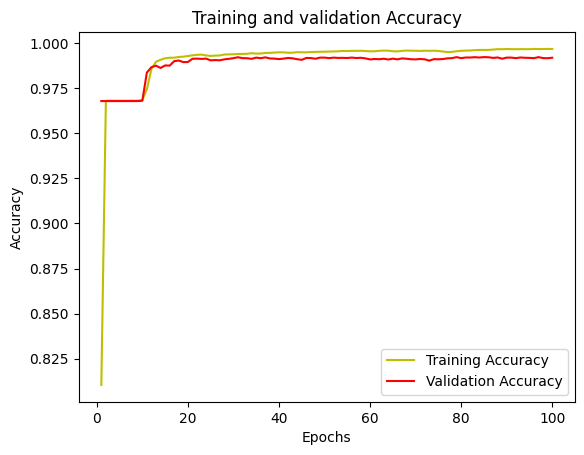
\includegraphics[scale=0.5]{bab4/acc-ori-unet.png} & 
			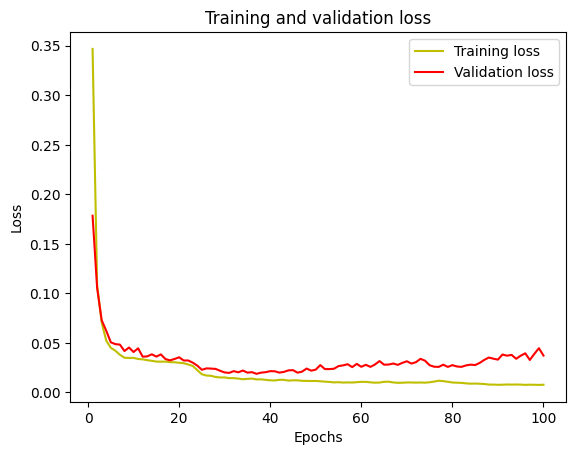
\includegraphics[scale=0.5]{bab4/loss-ori-unet.png} & \\
			(a) & (b)    % Caption untuk baris pertama
			% Caption untuk baris kedua
		\end{tabular}
		\caption{Nilai (a) akurasi dan (b) \textit{loss} segmentasi model U-Net yang tidak menggunakan filter reduksi \textit{noise}}
		\label{fig:performance-ori-unet}
	\end{figure}
	
	Kemudian hasil \textit{training} data 2D citra \textit{ultrasound} \textit{thrombus} dari hasil \textit{slice} citra 3D rekonstruksi yang tidak melalui tahap reduksi \textit{noise} menggunakan model segmentasi U-Net diperoleh sebagai berikut, (1) persentase nilai \textit{accuracy} sebesar 99,7392\%; (2) nilai \textit{loss} sebesar 0,0065; (3) nilai \textit{mean} IoU sebesar 0,8174; (4) nilai mean \textit{dice coefficient} sebesar 0,8923; serta (5) nilai \textit{mean hausdorff distance} sebesar 3,1244. Adapun grafik nilai \textit{accuracy} dan nilai \textit{loss} pada proses \textit{training} citra 2D \textit{ultrasound} \textit{thrombus} dari hasil citra 3D rekonstruksi yang tidak melalui tahap reduksi \textit{noise} menggunakan model segmentasi U-Net dapat dilihat pada Gambar \ref{fig:performance-ori-unet-rekonstruksi}.
	
	
	\begin{figure}[htbp]
		\centering
		\begin{tabular}{ccc}
			% Baris pertama dengan tiga gambar
			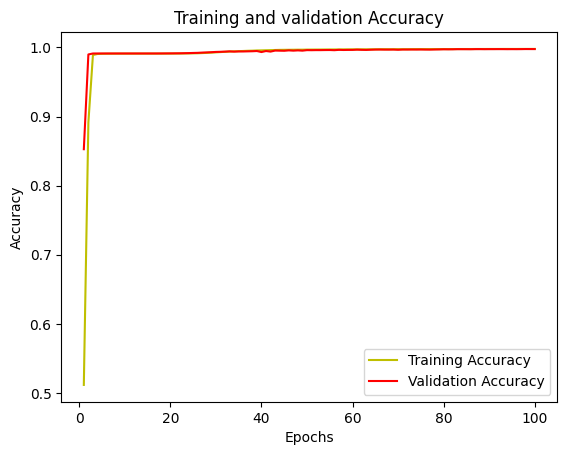
\includegraphics[scale=0.5]{bab4/Rekap Training/UNet/Ori/5/acc_99,75365400314331.png} &
			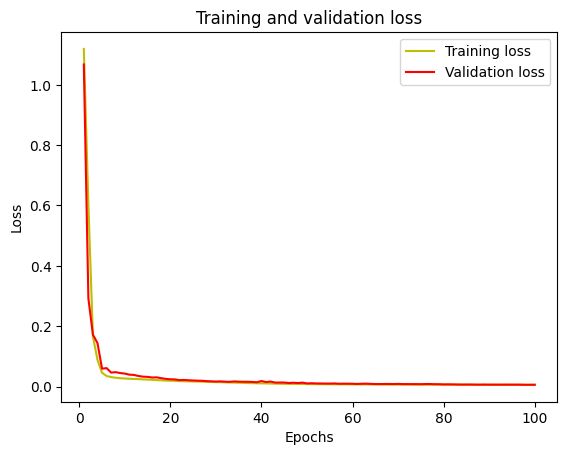
\includegraphics[scale=0.5]{bab4/Rekap Training/UNet/Ori/5/loss_0,0061.png} & \\
			(a) & (b)    % Caption untuk baris pertama
			% Caption untuk baris kedua
		\end{tabular}
		\caption{Nilai (a) akurasi dan (b) \textit{loss} segmentasi 2D citra \textit{ultrasound} \textit{thrombus} dari hasil citra 3D rekonstruksi yang tidak melalui tahap reduksi \textit{noise} menggunakan model U-Net.}
		\label{fig:performance-ori-unet-rekonstruksi}
	\end{figure}
	
	\item \textbf{Filter \textit{denoising} \textit{gaussian}} 
	
	Hasil \textit{training} model U-Net menggunakan citra 2D \textit{ultrasound} \textit{thrombus} dari 5 pasien penderita DVT yang telah melalui tahap reduksi \textit{noise} dengan menggunakan filter \textit{gaussian} diperoleh sebagai berikut, (1) persentase nilai \textit{accuracy} sebesar 99,166\%; (2) nilai \textit{loss} sebesar 0,0269; (3) persentase nilai \textit{mean} IoU sebesar 77,087\%; (4) nilai \textit{mean} \textit{dice coefficient} sebesar 0,8606; serta (5) nilai \textit{mean} \textit{hausdorff distance} sebesar 3,44. Adapun grafik nilai \textit{accuracy} dan nilai \textit{loss} pada proses \textit{training} citra 2D \textit{ultrasound} \textit{thrombus} dari 5 pasien penderita DVT yang telah melalui reduksi \textit{noise} menggunakan filter \textit{gaussian} dapat dilihat pada Gambar \ref{fig:performance-gaussian-unet} bagian a dan b.
	
	
	\begin{figure}[htbp]
		\centering
		\begin{tabular}{ccc}
			% Baris pertama dengan tiga gambar
			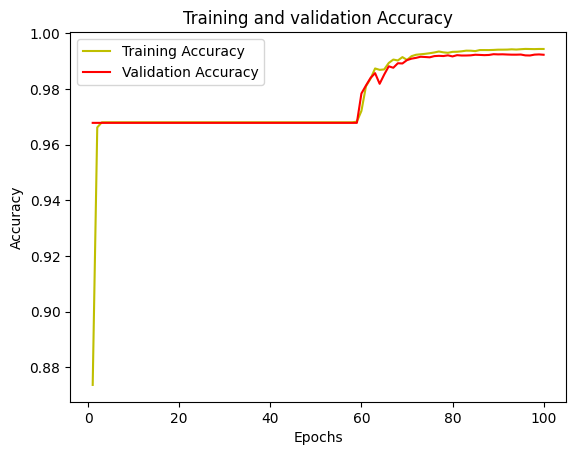
\includegraphics[scale=0.5]{bab4/acc-gaussian-unet.png} & 
			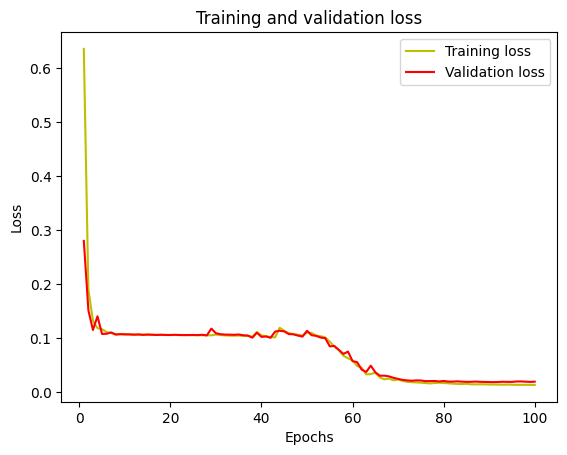
\includegraphics[scale=0.5]{bab4/loss-gaussian-unet.png} & \\
			(a) & (b)    % Caption untuk baris pertama
			% Caption untuk baris kedua
		\end{tabular}
		\caption{Nilai (a) akurasi dan (b) \textit{loss} segmentasi model U-Net yang menggunakan filter \textit{gaussian}}
		\label{fig:performance-gaussian-unet}
	\end{figure}
	
	Kemudian hasil \textit{training} data 2D citra \textit{ultrasound} \textit{thrombus} dari hasil \textit{slice} citra 3D rekonstruksi yang diberi filter \textit{denoising} \textit{gaussian} menggunakan model segmentasi U-Net diperoleh sebagai berikut, (1) persentase nilai \textit{accuracy} sebesar 99,6930\%; (2) nilai \textit{loss} sebesar 0,0074; (3) nilai \textit{mean} IoU sebesar 0,7965; (4) nilai mean \textit{dice coefficient} sebesar 0,8797; serta (5) nilai \textit{mean hausdorff distance} sebesar 5,0884. Adapun grafik nilai \textit{accuracy} dan nilai \textit{loss} pada proses \textit{training} citra 2D \textit{ultrasound} \textit{thrombus} dari hasil citra 3D rekonstruksi yang diberi filter \textit{denoising} \textit{gaussian} menggunakan model segmentasi U-Net dapat dilihat pada Gambar \ref{fig:performance-gaussian-unet-rekonstruksi}.
	
	
	\begin{figure}[htbp]
		\centering
		\begin{tabular}{ccc}
			% Baris pertama dengan tiga gambar
			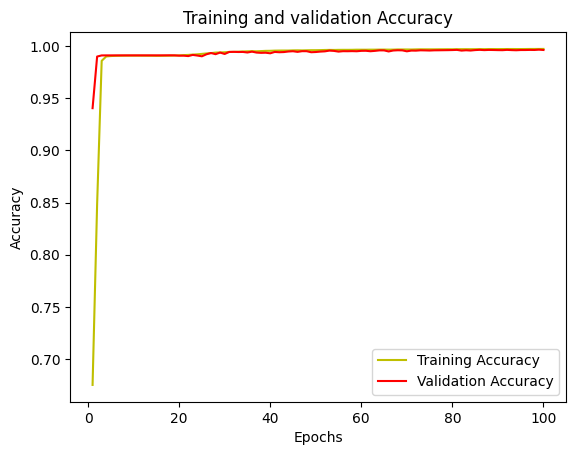
\includegraphics[scale=0.5]{bab4/Rekap Training/UNet/Gaussian/1/acc_99,63463544845581.png} &
			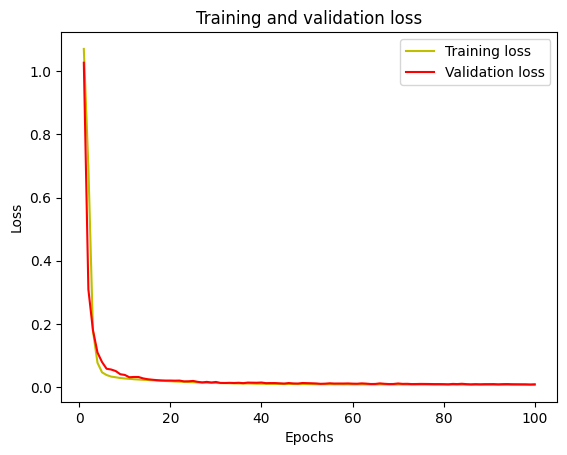
\includegraphics[scale=0.5]{bab4/Rekap Training/UNet/Gaussian/1/loss_0,0083.png} & \\
			(a) & (b)    % Caption untuk baris pertama
			% Caption untuk baris kedua
		\end{tabular}
		\caption{Nilai (a) akurasi dan (b) \textit{loss} segmentasi 2D citra \textit{ultrasound} \textit{thrombus} dari hasil citra 3D rekonstruksi yang yang diberi filter \textit{denoising} \textit{gaussian} menggunakan model U-Net.}
		\label{fig:performance-gaussian-unet-rekonstruksi}
	\end{figure}
	
	\item \textbf{Filter \textit{denoising} \textit{median}} 
	
	Hasil \textit{training} model U-Net menggunakan citra 2D \textit{ultrasound} \textit{thrombus} dari 5 pasien penderita DVT yang telah melalui tahap reduksi \textit{noise} dengan menggunakan filter \textit{median} diperoleh sebagai berikut, (1) persentase nilai \textit{accuracy} sebesar 99,131\%; (2) nilai \textit{loss} sebesar 0,0328; (3) persentase nilai \textit{mean} IoU sebesar 75,724\%; (4) nilai \textit{mean} \textit{dice coefficient} sebesar 0,8456; serta (5) nilai \textit{mean} \textit{hausdorff distance} sebesar 3,65. Adapun grafik nilai \textit{accuracy} dan nilai \textit{loss} pada proses \textit{training} citra 2D \textit{ultrasound} \textit{thrombus} dari 5 pasien penderita DVT yang telah melalui reduksi \textit{noise} menggunakan filter \textit{median} dapat dilihat pada Gambar \ref{fig:performance-median-unet} bagian a dan b.
	
	
	\begin{figure}[htbp]
		\centering
		\begin{tabular}{ccc}
			% Baris pertama dengan tiga gambar
			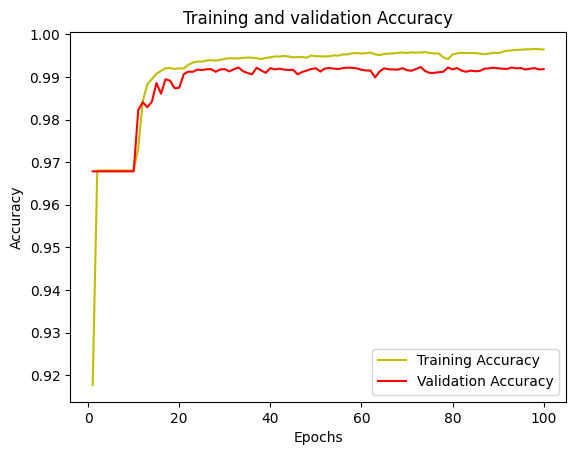
\includegraphics[scale=0.5]{bab4/acc-median-unet.png} & 
			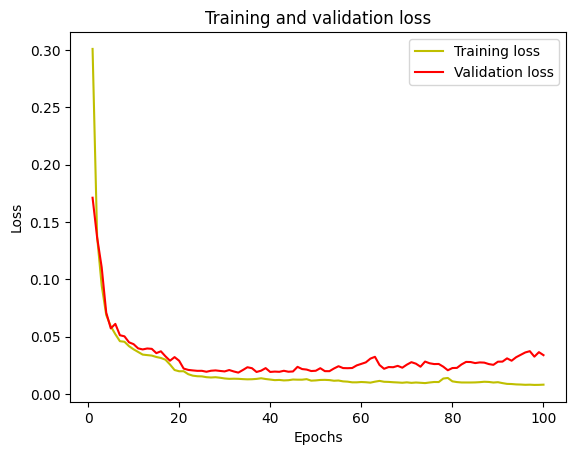
\includegraphics[scale=0.5]{bab4/loss-median-unet.png} & \\
			(a) & (b)    % Caption untuk baris pertama
			% Caption untuk baris kedua
		\end{tabular}
		\caption{Nilai (a) akurasi dan (b) \textit{loss} segmentasi model U-Net yang menggunakan filter \textit{median}}
		\label{fig:performance-median-unet}
	\end{figure}
	
	Hasil \textit{training} data 2D citra \textit{ultrasound} \textit{thrombus} dari hasil \textit{slice} citra 3D rekonstruksi yang diberi filter \textit{denoising} \textit{median} menggunakan model segmentasi U-Net diperoleh sebagai berikut, (1) persentase nilai \textit{accuracy} sebesar 99,7301\%; (2) nilai \textit{loss} sebesar 0,0067; (3) nilai \textit{mean} IoU sebesar 0,8023; (4) nilai mean \textit{dice coefficient} sebesar 0,8839; serta (5) nilai \textit{mean hausdorff distance} sebesar 5,0625. Adapun grafik nilai \textit{accuracy} dan nilai \textit{loss} pada proses \textit{training} citra 2D \textit{ultrasound} \textit{thrombus} dari hasil citra 3D rekonstruksi yang diberi filter \textit{denoising} \textit{median} menggunakan model segmentasi U-Net dapat dilihat pada Gambar \ref{fig:performance-median-unet-rekonstruksi}.
	
	
	\begin{figure}[htbp]
		\centering
		\begin{tabular}{ccc}
			% Baris pertama dengan tiga gambar
			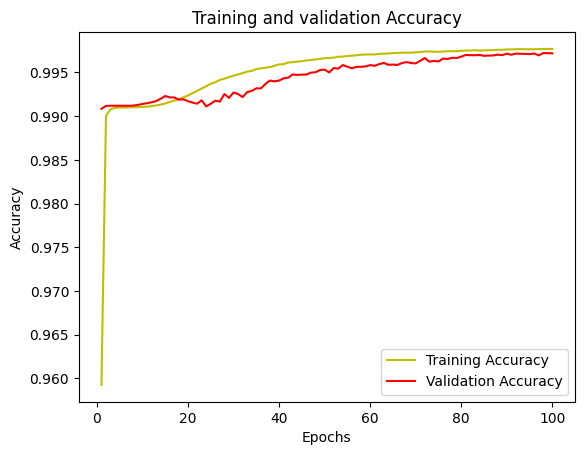
\includegraphics[scale=0.5]{bab4/Rekap Training/UNet/Median/5/acc_99,71805214881897.png} &
			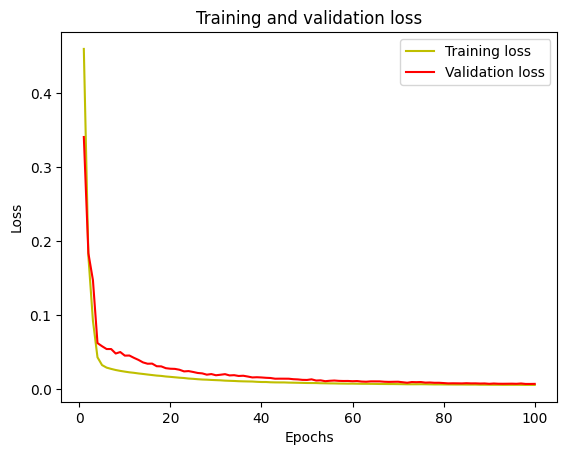
\includegraphics[scale=0.5]{bab4/Rekap Training/UNet/Median/5/loss_0,0070.png} & \\
			(a) & (b)    % Caption untuk baris pertama
			% Caption untuk baris kedua
		\end{tabular}
		\caption{Nilai (a) akurasi dan (b) \textit{loss} segmentasi 2D citra \textit{ultrasound} \textit{thrombus} dari hasil citra 3D rekonstruksi yang yang diberi filter \textit{denoising} \textit{median} menggunakan model U-Net.}
		\label{fig:performance-median-unet-rekonstruksi}
	\end{figure}
	
	
	\item \textbf{Filter \textit{denoising} \textit{mean}} 
	
	Hasil \textit{training} model U-Net menggunakan citra 2D \textit{ultrasound} \textit{thrombus} dari 5 pasien penderita DVT yang telah melalui tahap reduksi \textit{noise} dengan menggunakan filter \textit{mean} diperoleh sebagai berikut, (1) persentase nilai \textit{accuracy} sebesar 98,374\%; (2) nilai \textit{loss} sebesar 0,0305; (3) persentase nilai \textit{mean} IoU sebesar 71,476\%; (4) nilai \textit{mean} \textit{dice coefficient} sebesar 0,8570; serta (5) nilai \textit{mean} \textit{hausdorff distance} sebesar 3,72. Adapun grafik nilai \textit{accuracy} dan nilai \textit{loss} pada proses \textit{training} citra 2D \textit{ultrasound} \textit{thrombus} dari 5 pasien penderita DVT yang telah melalui reduksi \textit{noise} menggunakan filter \textit{mean} dapat dilihat Gambar \ref{fig:performance-mean-unet} bagian a dan b.
	
	
	\begin{figure}[H]
		\centering
		\begin{tabular}{ccc}
			% Baris pertama dengan tiga gambar
			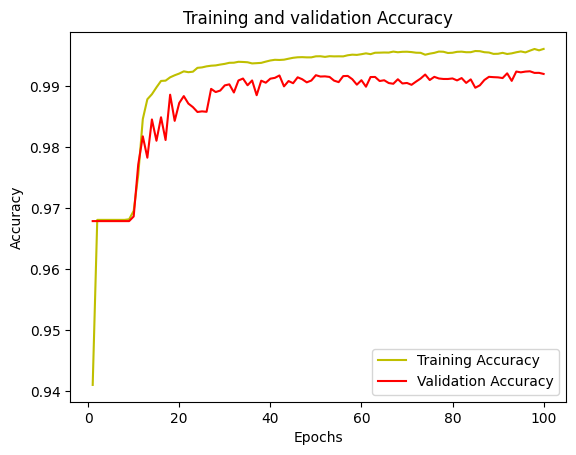
\includegraphics[scale=0.4]{bab4/acc-mean-unet.png} & 
			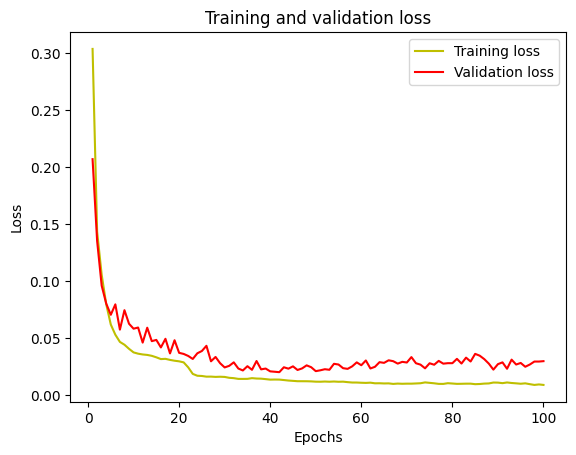
\includegraphics[scale=0.4]{bab4/loss-mean-unet.png} & \\
			(a) & (b)    % Caption untuk baris pertama
			% Caption untuk baris kedua
		\end{tabular}
		\caption{Nilai (a) akurasi dan (b) \textit{loss} segmentasi model U-Net yang menggunakan filter \textit{mean}}
		\label{fig:performance-mean-unet}
	\end{figure}
	
	
	Hasil \textit{training} data 2D citra \textit{ultrasound} \textit{thrombus} dari hasil \textit{slice} citra 3D rekonstruksi yang diberi filter \textit{denoising} \textit{mean} menggunakan model segmentasi U-Net diperoleh sebagai berikut, (1) persentase nilai \textit{accuracy} sebesar 99,7170\%; (2) nilai \textit{loss} sebesar 0,0068; (3) nilai \textit{mean} IoU sebesar 0,8147; (4) nilai mean \textit{dice coefficient} sebesar 0,8925; serta (5) nilai \textit{mean hausdorff distance} sebesar 5,2611. Adapun grafik nilai \textit{accuracy} dan nilai \textit{loss} pada proses \textit{training} citra 2D \textit{ultrasound} \textit{thrombus} dari hasil citra 3D rekonstruksi yang diberi filter \textit{denoising} \textit{mean} menggunakan model segmentasi U-Net dapat dilihat pada Gambar \ref{fig:performance-mean-unet-rekonstruksi}.
	
	
	\begin{figure}[htbp]
		\centering
		\begin{tabular}{ccc}
			% Baris pertama dengan tiga gambar
			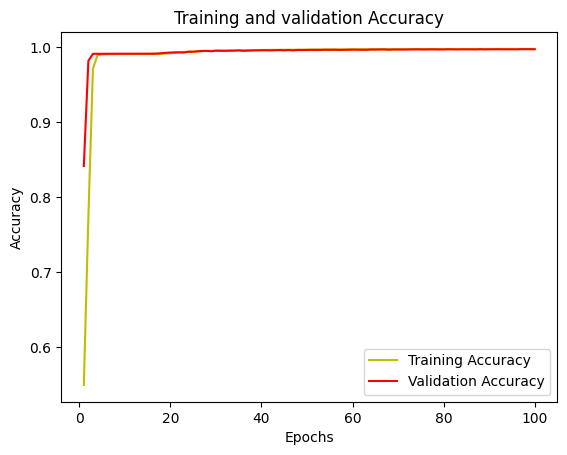
\includegraphics[scale=0.4]{bab4/Rekap Training/UNet/Mean/3/acc_99,71330165863037.png} &
			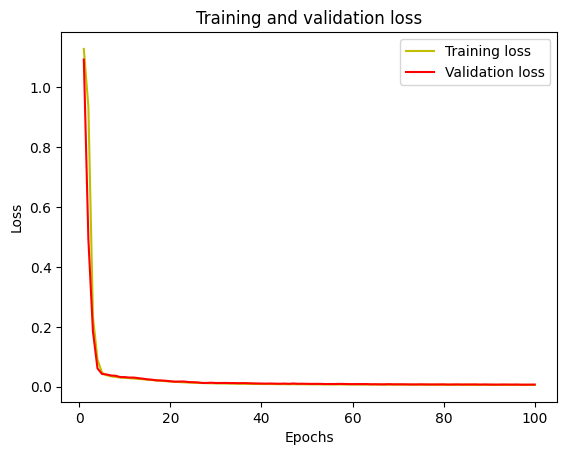
\includegraphics[scale=0.4]{bab4/Rekap Training/UNet/Mean/3/loss_0,0069.png} & \\
			(a) & (b)    % Caption untuk baris pertama
			% Caption untuk baris kedua
		\end{tabular}
		\caption{Nilai (a) akurasi dan (b) \textit{loss} segmentasi 2D citra \textit{ultrasound} \textit{thrombus} dari hasil citra 3D rekonstruksi yang yang diberi filter \textit{denoising} \textit{mean} menggunakan model U-Net.}
		\label{fig:performance-mean-unet-rekonstruksi}
	\end{figure}
	
	\item \textbf{Filter \textit{denoising} \textit{bilateral}}
	
	Hasil \textit{training} model U-Net menggunakan citra 2D \textit{ultrasound} \textit{thrombus} dari 5 pasien penderita DVT yang telah melalui tahap reduksi \textit{noise} dengan menggunakan filter \textit{bilateral} diperoleh sebagai berikut, (1) persentase nilai \textit{accuracy} sebesar 98,378\%; (2) nilai \textit{loss} sebesar 0,0267; (3) persentase nilai \textit{mean} IoU sebesar 72,327\%; (4) nilai \textit{mean} \textit{dice coefficient} sebesar 0,8589; serta (5) nilai \textit{mean} \textit{hausdorff distance} sebesar 3,58. Adapun grafik nilai \textit{accuracy} dan nilai \textit{loss} pada proses \textit{training} citra 2D \textit{ultrasound} \textit{thrombus} dari 5 pasien penderita DVT yang telah melalui reduksi \textit{noise} menggunakan filter \textit{bilateral} dapat dilihat pada Gambar \ref{fig:performance-bilateral-unet} bagian a dan b.
	
	
	\begin{figure}[htbp]
		\centering
		\begin{tabular}{ccc}
			% Baris pertama dengan tiga gambar
			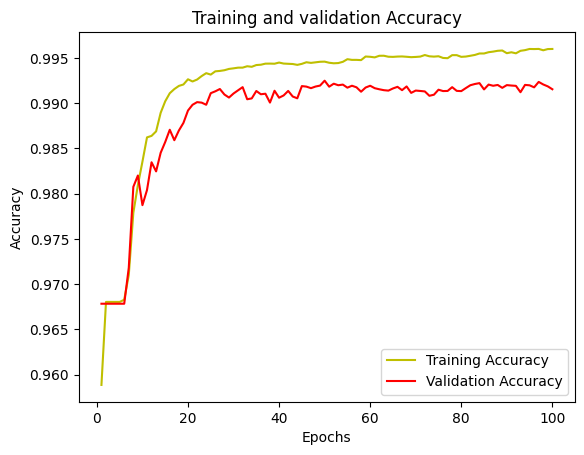
\includegraphics[scale=0.5]{bab4/acc-bilateral-unet.png} & 
			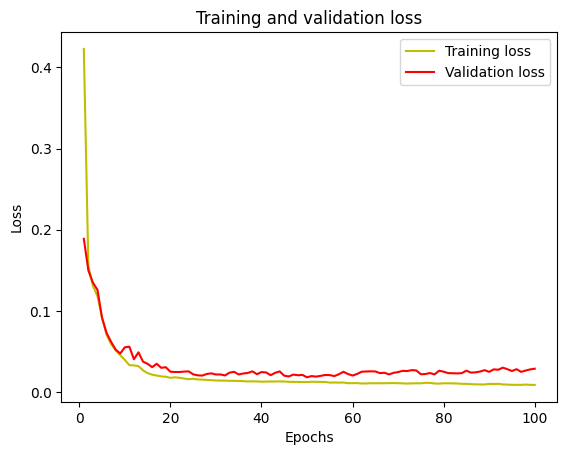
\includegraphics[scale=0.5]{bab4/loss-bilateral-unet.png} & \\
			(a)&(b)    % Caption untuk baris pertama
			% Caption untuk baris kedua
		\end{tabular}
		\caption{Nilai (a) akurasi dan (b) \textit{loss} segmentasi model U-Net yang menggunakan filter \textit{bilateral}}
		\label{fig:performance-bilateral-unet}
	\end{figure}
	
	Hasil \textit{training} data 2D citra \textit{ultrasound} \textit{thrombus} dari hasil \textit{slice} citra 3D rekonstruksi yang diberi filter \textit{denoising} \textit{bilateral} menggunakan model segmentasi U-Net diperoleh sebagai berikut, (1) persentase nilai \textit{accuracy} sebesar 99,7318\%; (2) nilai \textit{loss} sebesar 0,0066; (3) nilai \textit{mean} IoU sebesar 0,8070; (4) nilai mean \textit{dice coefficient} sebesar 0,8872; serta (5) nilai \textit{mean hausdorff distance} sebesar 6,6663. Adapun grafik nilai \textit{accuracy} dan nilai \textit{loss} pada proses \textit{training} citra 2D \textit{ultrasound} \textit{thrombus} dari hasil citra 3D rekonstruksi yang diberi filter \textit{denoising} \textit{bilateral} menggunakan model segmentasi U-Net dapat dilihat pada Gambar \ref{fig:performance-bilateral-unet-rekonstruksi}.
	
	
	\begin{figure}[htbp]
		\centering
		\begin{tabular}{ccc}
			% Baris pertama dengan tiga gambar
			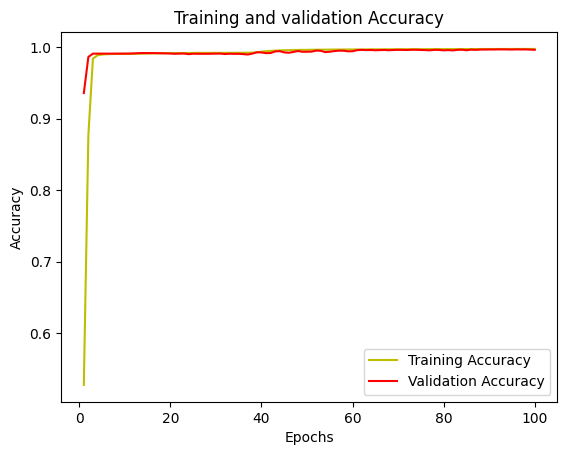
\includegraphics[scale=0.5]{bab4/Rekap Training/UNet/Bilateral/5/acc_99,65311884880066.png} &
			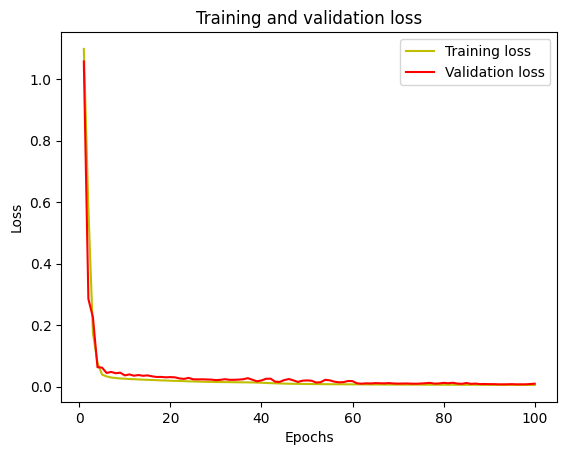
\includegraphics[scale=0.5]{bab4/Rekap Training/UNet/Bilateral/5/loss_0,0096.png} & \\
			(a) & (b)    % Caption untuk baris pertama
			% Caption untuk baris kedua
		\end{tabular}
		\caption{Nilai (a) akurasi dan (b) \textit{loss} segmentasi 2D citra \textit{ultrasound} \textit{thrombus} dari hasil citra 3D rekonstruksi yang yang diberi filter \textit{denoising} \textit{bilateral} menggunakan model U-Net.}
		\label{fig:performance-bilateral-unet-rekonstruksi}
	\end{figure}
	
	\item \textbf{Filter \textit{denoising} \textit{non local means}}
	
	Hasil \textit{training} model U-Net menggunakan citra 2D \textit{ultrasound} \textit{thrombus} dari 5 pasien penderita DVT yang telah melalui tahap reduksi \textit{noise} dengan menggunakan filter \textit{non local means} diperoleh sebagai berikut, (1) persentase nilai \textit{accuracy} sebesar 98,381\%; (2) nilai \textit{loss} sebesar 0,0272; (3) persentase nilai \textit{mean} IoU sebesar 71,345\%; (4) nilai \textit{mean} \textit{dice coefficient} sebesar 0,8599; serta (5) nilai \textit{mean} \textit{hausdorff distance} sebesar 3,73. Adapun grafik nilai \textit{accuracy} dan nilai \textit{loss} pada proses \textit{training} citra 2D \textit{ultrasound} \textit{thrombus} dari 5 pasien penderita DVT yang telah melalui reduksi \textit{noise} menggunakan filter \textit{non local means} dapat dilihat pada Gambar \ref{fig:performance-nlm-unet} bagian a dan b.
	
	
	\begin{figure}[htbp]
		\centering
		\begin{tabular}{ccc}
			% Baris pertama dengan tiga gambar
			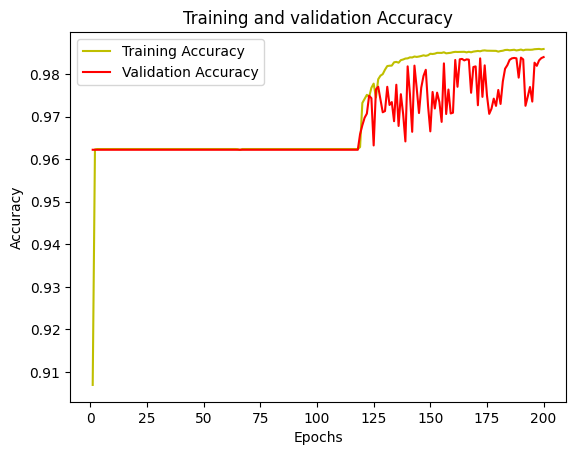
\includegraphics[scale=0.5]{bab4/acc-nlm-unet.png} & 
			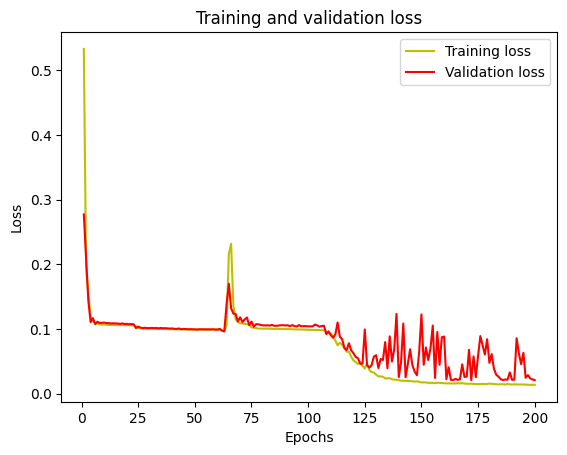
\includegraphics[scale=0.5]{bab4/loss-nlm-unet.png} & \\
			(a) & (b)    % Caption untuk baris pertama
			% Caption untuk baris kedua
		\end{tabular}
		\caption{Nilai (a) akurasi dan (b) \textit{loss} segmentasi model U-Net yang menggunakan filter \textit{non local means}}
		\label{fig:performance-nlm-unet}
	\end{figure}
	
	
	Hasil \textit{training} data 2D citra \textit{ultrasound} \textit{thrombus} dari hasil \textit{slice} citra 3D rekonstruksi yang diberi filter \textit{denoising} \textit{non local means} menggunakan model segmentasi U-Net diperoleh sebagai berikut, (1) persentase nilai \textit{accuracy} sebesar 99,6598\%; (2) nilai \textit{loss} sebesar 0,0082; (3) nilai \textit{mean} IoU sebesar 0,7819; (4) nilai mean \textit{dice coefficient} sebesar 0,8697; serta (5) nilai \textit{mean hausdorff distance} sebesar 4,0778. Adapun grafik nilai \textit{accuracy} dan nilai \textit{loss} pada proses \textit{training} citra 2D \textit{ultrasound} \textit{thrombus} dari hasil citra 3D rekonstruksi yang diberi filter \textit{denoising} \textit{non local means} menggunakan model segmentasi U-Net dapat dilihat pada Gambar \ref{fig:performance-nlm-unet-rekonstruksi}.
	
	
	\begin{figure}[htbp]
		\centering
		\begin{tabular}{ccc}
			% Baris pertama dengan tiga gambar
			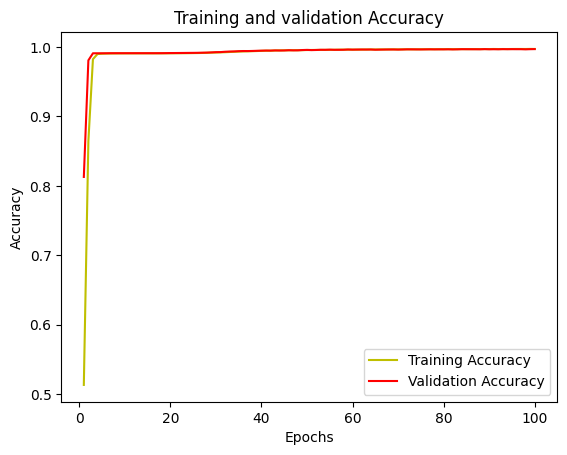
\includegraphics[scale=0.5]{bab4/Rekap Training/UNet/Nlm/1/acc_99,70923662185669.png} &
			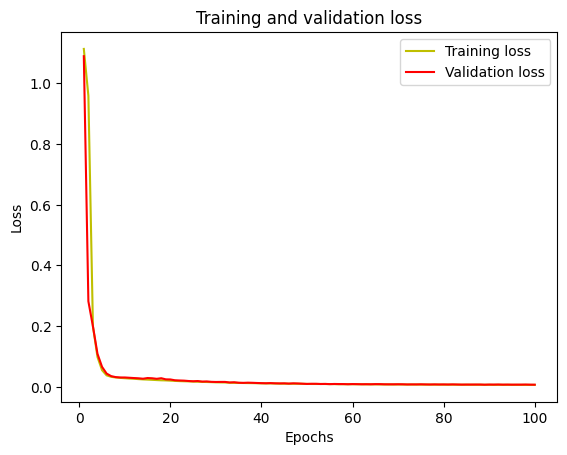
\includegraphics[scale=0.5]{bab4/Rekap Training/UNet/Nlm/1/loss_0,0070.png} & \\
			(a) & (b)    % Caption untuk baris pertama
			% Caption untuk baris kedua
		\end{tabular}
		\caption{Nilai (a) akurasi dan (b) \textit{loss} segmentasi 2D citra \textit{ultrasound} \textit{thrombus} dari hasil citra 3D rekonstruksi yang yang diberi filter \textit{denoising} \textit{non local means} menggunakan model U-Net.}
		\label{fig:performance-nlm-unet-rekonstruksi}
	\end{figure}
	
\end{enumerate}


\subsubsection{Training Model U-Net dengan \textit{Encoder} \textit{Pre-trained} VGG16}

\begin{enumerate}
	\item \textbf{Citra 2D tanpa diberi filter \textit{denoising}}
	
	Hasil \textit{training} model U-Net yang telah dimodifikasi bagian \textit{encoder}nya menggunakan model \textit{pre-trained} VGG16 dengan menggunakan citra 2D \textit{ultrasound} \textit{thrombus} dari 5 pasien penderita DVT yang tidak melalui tahap reduksi \textit{noise} diperoleh sebagai berikut, (1) persentase nilai \textit{accuracy} sebesar 99,188\%; (2) nilai \textit{loss} sebesar 0,0358; (3) persentase nilai \textit{mean} IoU sebesar 87,086\%; (4) nilai \textit{mean} \textit{dice coefficient} sebesar 0,8677; serta (5) nilai \textit{mean} \textit{hausdorff distance} sebesar 3,11. Adapun grafik nilai \textit{accuracy} dan nilai \textit{loss} pada proses \textit{training} citra 2D \textit{ultrasound} \textit{thrombus} dari 5 pasien penderita DVT yang tidak melalui tahap reduksi \textit{noise} dapat dilihat pada Gambar \ref{fig:performance-ori-vggunet} bagian a dan b.
	
	
	\begin{figure}[htbp]
		\centering
		\begin{tabular}{ccc}
			% Baris pertama dengan tiga gambar
			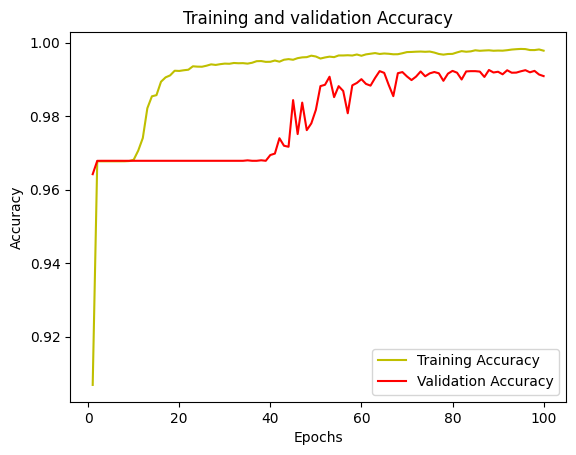
\includegraphics[scale=0.5]{bab4/acc-ori-vggunet.png} &
			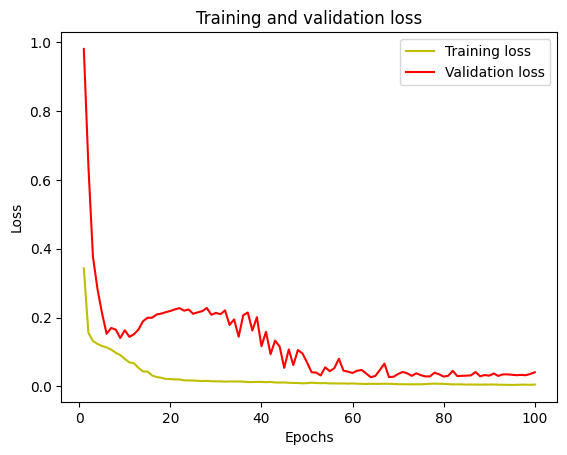
\includegraphics[scale=0.5]{bab4/loss-ori-vggunet.png} & \\
			(a) & (b)    % Caption untuk baris pertama
			% Caption untuk baris kedua
		\end{tabular}
		\caption{Nilai (a) akurasi dan (b) \textit{loss} segmentasi model \textit{pre-trained} VGG16-UNet yang tidak menggunakan filter reduksi \textit{noise}}
		\label{fig:performance-ori-vggunet}
	\end{figure}
	
	
	Hasil \textit{training} data 2D citra \textit{ultrasound} \textit{thrombus} dari hasil \textit{slice} citra 3D rekonstruksi yang tidak melalui tahap reduksi \textit{noise} menggunakan model \textit{pre-trained} VGG16 dan U-Net diperoleh sebagai berikut, (1) persentase nilai \textit{accuracy} sebesar 99,7591\%; (2) nilai \textit{loss} sebesar 0,0103; (3) nilai \textit{mean} IoU sebesar 0,8302; (4) nilai mean \textit{dice coefficient} sebesar 0,9028; serta (5) nilai \textit{mean hausdorff distance} sebesar 2,0790. Adapun grafik nilai \textit{accuracy} dan nilai \textit{loss} pada proses \textit{training} citra 2D \textit{ultrasound} \textit{thrombus} dari hasil citra 3D rekonstruksi yang tidak melalui tahap reduksi \textit{noise} menggunakan \textit{pre-trained} VGG16 dan U-Net dapat dilihat pada Gambar \ref{fig:performance-ori-vggunet-rekonstruksi}.
	
	
	\begin{figure}[htbp]
		\centering
		\begin{tabular}{ccc}
			% Baris pertama dengan tiga gambar
			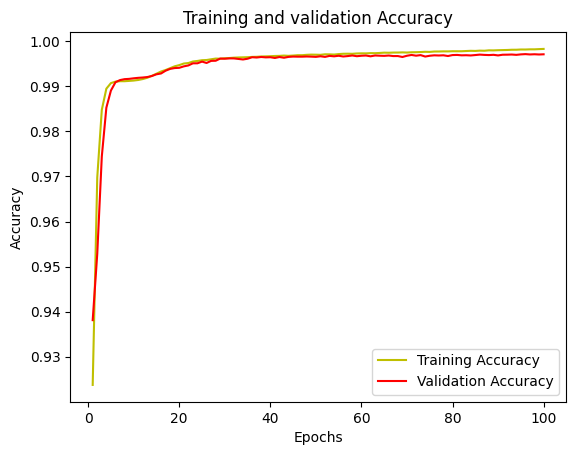
\includegraphics[scale=0.5]{bab4/Rekap Training/VGG16-UNet/Ori/5/acc_99,71024990081787.png} &
			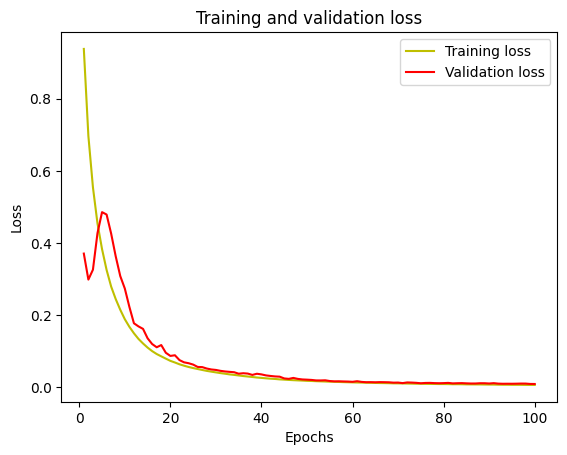
\includegraphics[scale=0.5]{bab4/Rekap Training/VGG16-UNet/Ori/5/loss_0,0089.png} & \\
			(a) & (b)    % Caption untuk baris pertama
			% Caption untuk baris kedua
		\end{tabular}
		\caption{Nilai (a) akurasi dan (b) \textit{loss} segmentasi 2D citra \textit{ultrasound} \textit{thrombus} dari hasil citra 3D rekonstruksi yang tidak melalui tahap reduksi \textit{noise} menggunakan model \textit{pre-trained} VGG16 dan U-Net.}
		\label{fig:performance-ori-vggunet-rekonstruksi}
	\end{figure}
	
	\item \textbf{Filter \textit{denoising} \textit{gaussian}}
	
	Hasil \textit{training} model U-Net yang telah dimodifikasi bagian \textit{encoder}nya menggunakan model \textit{pre-trained} VGG16 dengan menggunakan citra 2D \textit{ultrasound} \textit{thrombus} dari 5 pasien penderita DVT yang melalui tahap reduksi \textit{noise} menggunakan filter \textit{gaussian} diperoleh sebagai berikut, (1) persentase nilai \textit{accuracy} sebesar 99,222\%; (2) nilai \textit{loss} sebesar 0,0284; (3) persentase nilai \textit{mean} IoU sebesar 88,298\%; (4) nilai \textit{mean} \textit{dice coefficient} sebesar 0,8784; serta (5) nilai \textit{mean} \textit{hausdorff distance} sebesar 3,07. Adapun grafik nilai \textit{accuracy} dan nilai \textit{loss} pada proses \textit{training} citra 2D \textit{ultrasound} \textit{thrombus} dari 5 pasien penderita DVT yang melalui tahap reduksi \textit{noise} menggunakan filter \textit{gaussian} dapat dilihat pada Gambar \ref{fig:performance-gaussian-vggunet} bagian a dan b.
	
	
	\begin{figure}[htbp]
		\centering
		\begin{tabular}{ccc}
			% Baris pertama dengan tiga gambar
			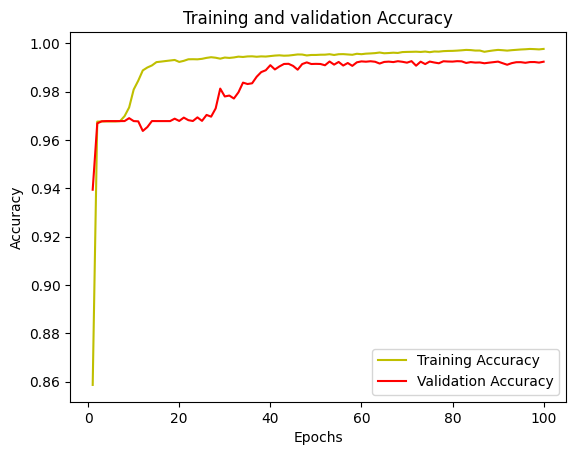
\includegraphics[scale=0.5]{bab4/acc-gaussian-vggunet.png} &
			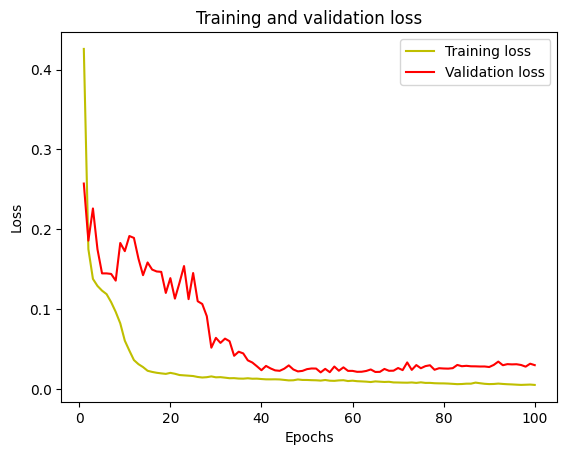
\includegraphics[scale=0.5]{bab4/loss-gaussian-vggunet.png} & \\
			(a) & (b)    % Caption untuk baris pertama
			% Caption untuk baris kedua
		\end{tabular}
		\caption{Nilai (a) akurasi dan (b) \textit{loss} segmentasi model \textit{pre-trained} VGG16-UNet yang menggunakan filter \textit{gaussian}}
		\label{fig:performance-gaussian-vggunet}
	\end{figure}
	
	Hasil \textit{training} data 2D citra \textit{ultrasound} \textit{thrombus} dari hasil \textit{slice} citra 3D rekonstruksi yang diberi filter \textit{denoising} \textit{gaussian} model \textit{pre-trained} VGG16 dan U-Net diperoleh sebagai berikut, (1) persentase nilai \textit{accuracy} sebesar 99,7489\%; (2) nilai \textit{loss} sebesar 0,00947; (3) nilai \textit{mean} IoU sebesar 0,8267; (4) nilai mean \textit{dice coefficient} sebesar 0,9004; serta (5) nilai \textit{mean hausdorff distance} sebesar 1,9526. Adapun grafik nilai \textit{accuracy} dan nilai \textit{loss} pada proses \textit{training} citra 2D \textit{ultrasound} \textit{thrombus} dari hasil citra 3D rekonstruksi yang diberi filter \textit{denoising} \textit{gaussian} menggunakan model model \textit{pre-trained} VGG16 dan U-Net dapat dilihat pada Gambar \ref{fig:performance-gaussian-vggunet-rekonstruksi}.
	
	
	\begin{figure}[htbp]
		\centering
		\begin{tabular}{ccc}
			% Baris pertama dengan tiga gambar
			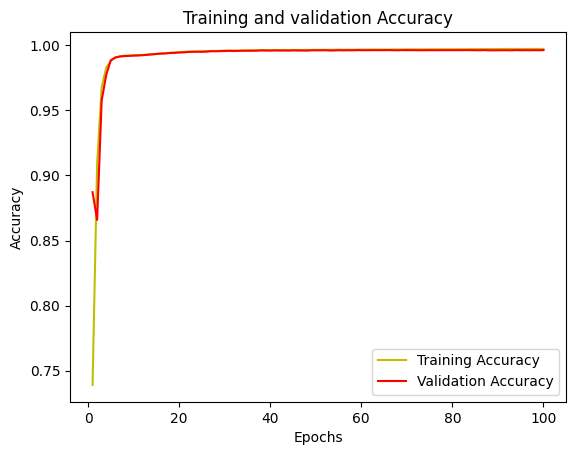
\includegraphics[scale=0.5]{bab4/Rekap Training/VGG16-UNet/gaussian/3/acc_99,63209629058838.png} &
			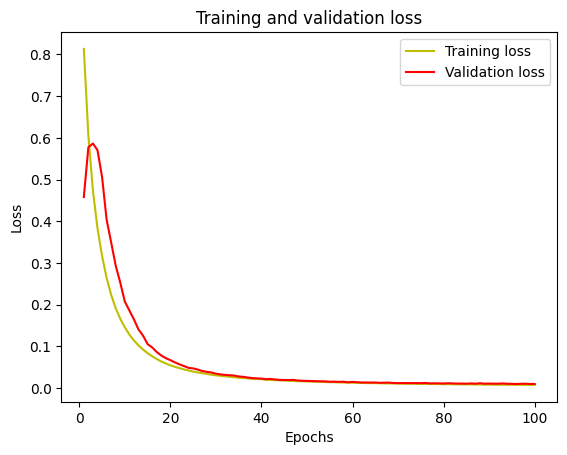
\includegraphics[scale=0.5]{bab4/Rekap Training/VGG16-UNet/gaussian/3/loss_0,0098.png} & \\
			(a) & (b)    % Caption untuk baris pertama
			% Caption untuk baris kedua
		\end{tabular}
		\caption{Nilai (a) akurasi dan (b) \textit{loss} segmentasi 2D citra \textit{ultrasound} \textit{thrombus} dari hasil citra 3D rekonstruksi yang yang diberi filter \textit{denoising} \textit{gaussian} menggunakan model \textit{pre-trained} VGG16 dan U-Net.}
		\label{fig:performance-gaussian-vggunet-rekonstruksi}
	\end{figure}
	
	\item \textbf{Filter \textit{denoising} \textit{median}}
	
	Hasil \textit{training} model U-Net yang telah dimodifikasi bagian \textit{encoder}nya menggunakan model \textit{pre-trained} VGG16 dengan menggunakan citra 2D \textit{ultrasound} \textit{thrombus} dari 5 pasien penderita DVT yang melalui tahap reduksi \textit{noise} menggunakan filter \textit{median} diperoleh sebagai berikut, (1) persentase nilai \textit{accuracy} sebesar 99,204\%; (2) nilai \textit{loss} sebesar 0,0353; (3) persentase nilai \textit{mean} IoU sebesar 86,624\%; (4) nilai \textit{mean} \textit{dice coefficient} sebesar 0,8720; serta (5) nilai \textit{mean} \textit{hausdorff distance} sebesar 3,12. Adapun grafik nilai \textit{accuracy} dan nilai \textit{loss} pada proses \textit{training} citra 2D \textit{ultrasound} \textit{thrombus} dari 5 pasien penderita DVT yang melalui tahap reduksi \textit{noise} menggunakan filter \textit{median} dapat dilihat pada Gambar \ref{fig:performance-median-vggunet} bagian a dan b.
	
	
	\begin{figure}[htbp]
		\centering
		\begin{tabular}{ccc}
			% Baris pertama dengan tiga gambar
			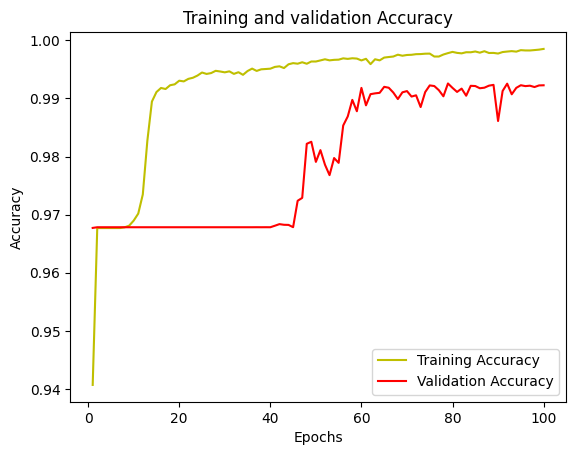
\includegraphics[scale=0.5]{bab4/acc-median-vggunet.png} &
			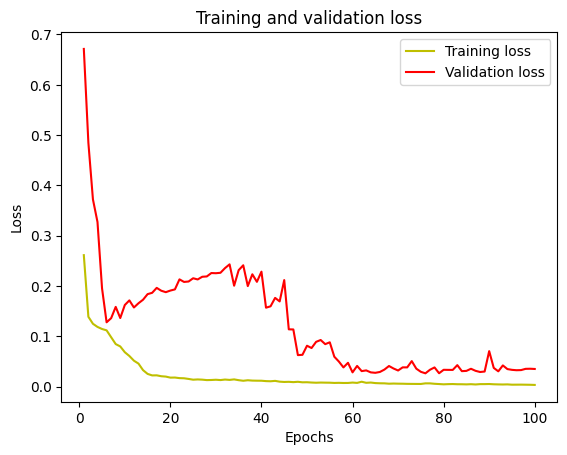
\includegraphics[scale=0.5]{bab4/loss-median-vggunet.png} & \\
			(a) & (b)    % Caption untuk baris pertama
			% Caption untuk baris kedua
		\end{tabular}
		\caption{Nilai (a) akurasi dan (b) \textit{loss} segmentasi model \textit{pre-trained} VGG16-UNet yang menggunakan filter \textit{median}}
		\label{fig:performance-median-vggunet}
	\end{figure}
	
	
	Hasil \textit{training} data 2D citra \textit{ultrasound} \textit{thrombus} dari hasil \textit{slice} citra 3D rekonstruksi yang diberi filter \textit{denoising} \textit{median} model \textit{pre-trained} VGG16 dan U-Net diperoleh sebagai berikut, (1) persentase nilai \textit{accuracy} sebesar 99,7512\%; (2) nilai \textit{loss} sebesar 0,00953; (3) nilai \textit{mean} IoU sebesar 0,8336; (4) nilai mean \textit{dice coefficient} sebesar 0,9049; serta (5) nilai \textit{mean hausdorff distance} sebesar 2,0071. Adapun grafik nilai \textit{accuracy} dan nilai \textit{loss} pada proses \textit{training} citra 2D \textit{ultrasound} \textit{thrombus} dari hasil citra 3D rekonstruksi yang diberi filter \textit{denoising} \textit{median} menggunakan model model \textit{pre-trained} VGG16 dan U-Net dapat dilihat pada Gambar \ref{fig:performance-median-vggunet-rekonstruksi}.
	
	
	\begin{figure}[htbp]
		\centering
		\begin{tabular}{ccc}
			% Baris pertama dengan tiga gambar
			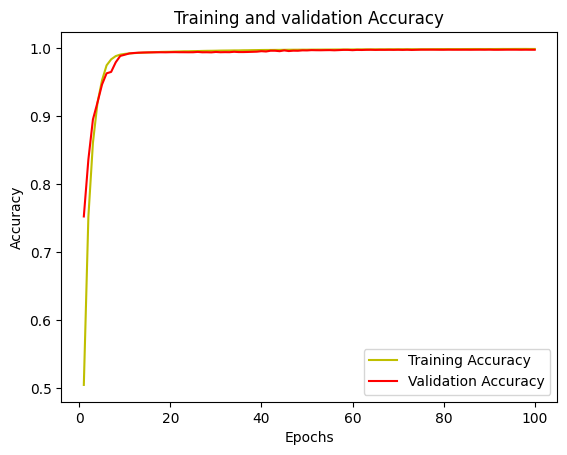
\includegraphics[scale=0.5]{bab4/Rekap Training/VGG16-UNet/median/3/acc_99,74772334098816.png} &
			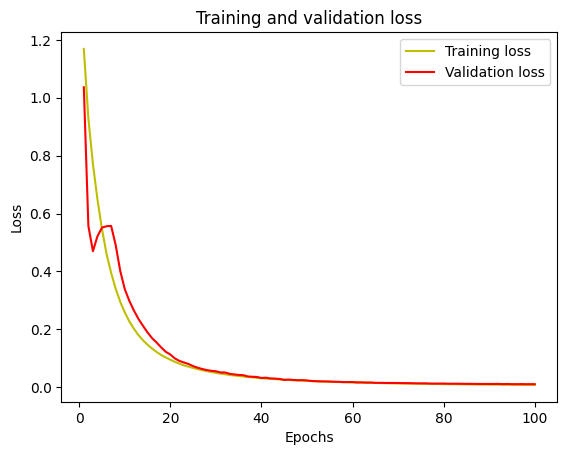
\includegraphics[scale=0.5]{bab4/Rekap Training/VGG16-UNet/median/3/loss_0,0101.png} & \\
			(a) & (b)    % Caption untuk baris pertama
			% Caption untuk baris kedua
		\end{tabular}
		\caption{Nilai (a) akurasi dan (b) \textit{loss} segmentasi 2D citra \textit{ultrasound} \textit{thrombus} dari hasil citra 3D rekonstruksi yang yang diberi filter \textit{denoising} \textit{median} menggunakan model \textit{pre-trained} VGG16 dan U-Net.}
		\label{fig:performance-median-vggunet-rekonstruksi}
	\end{figure}
	

	\item \textbf{Filter \textit{denoising} \textit{mean}}
	
	Hasil \textit{training} model U-Net yang telah dimodifikasi bagian \textit{encoder}nya menggunakan model \textit{pre-trained} VGG16 dengan menggunakan citra 2D \textit{ultrasound} \textit{thrombus} dari 5 pasien penderita DVT yang melalui tahap reduksi \textit{noise} menggunakan filter \textit{mean} diperoleh sebagai berikut, (1) persentase nilai \textit{accuracy} sebesar 99,218\%; (2) nilai \textit{loss} sebesar 0,0256; (3) persentase nilai \textit{mean} IoU sebesar 88,088\%; (4) nilai \textit{mean} \textit{dice coefficient} sebesar 0,8764; serta (5) nilai \textit{mean} \textit{hausdorff distance} sebesar 3,48. Adapun grafik nilai \textit{accuracy} dan nilai \textit{loss} pada proses \textit{training} citra 2D \textit{ultrasound} \textit{thrombus} dari 5 pasien penderita DVT yang melalui tahap reduksi \textit{noise} menggunakan filter \textit{mean} dapat dilihat pada Gambar \ref{fig:performance-mean-vggunet} bagian a dan b.
	
	
	\begin{figure}[htbp]
		\centering
		\begin{tabular}{ccc}
			% Baris pertama dengan tiga gambar
			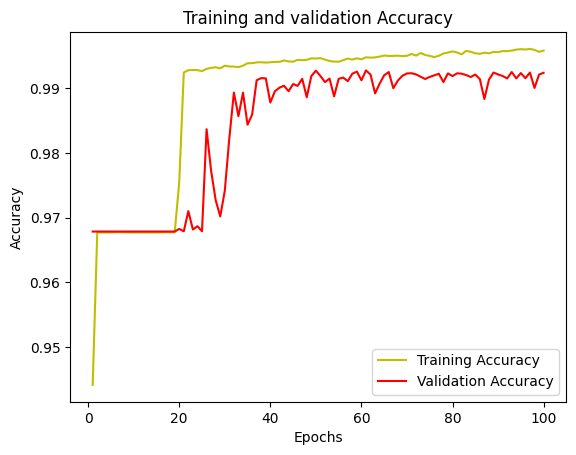
\includegraphics[scale=0.5]{bab4/acc-mean-vggunet.png} &
			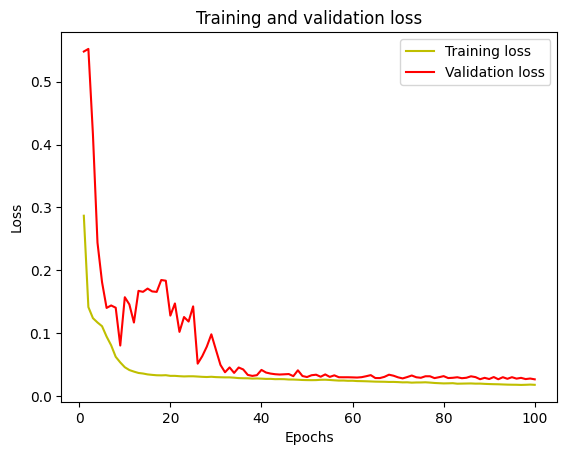
\includegraphics[scale=0.5]{bab4/loss-mean-vggunet.png} & \\
			(a) & (b)    % Caption untuk baris pertama
			% Caption untuk baris kedua
		\end{tabular}
		\caption{Nilai (a) akurasi dan (b) \textit{loss} segmentasi model \textit{pre-trained} VGG16-UNet yang menggunakan filter \textit{mean}}
		\label{fig:performance-mean-vggunet}
	\end{figure}
	
	
	Hasil \textit{training} data 2D citra \textit{ultrasound} \textit{thrombus} dari hasil \textit{slice} citra 3D rekonstruksi yang diberi filter \textit{denoising} \textit{mean} model \textit{pre-trained} VGG16 dan U-Net diperoleh sebagai berikut, (1) persentase nilai \textit{accuracy} sebesar 99,7480\%; (2) nilai \textit{loss} sebesar 0,00950; (3) nilai \textit{mean} IoU sebesar 0,8248; (4) nilai mean \textit{dice coefficient} sebesar 0,8992; serta (5) nilai \textit{mean hausdorff distance} sebesar 2,1718. Adapun grafik nilai \textit{accuracy} dan nilai \textit{loss} pada proses \textit{training} citra 2D \textit{ultrasound} \textit{thrombus} dari hasil citra 3D rekonstruksi yang diberi filter \textit{denoising} \textit{mean} menggunakan model model \textit{pre-trained} VGG16 dan U-Net dapat dilihat pada Gambar \ref{fig:performance-mean-vggunet-rekonstruksi}.
	
	
	\begin{figure}[htbp]
		\centering
		\begin{tabular}{ccc}
			% Baris pertama dengan tiga gambar
			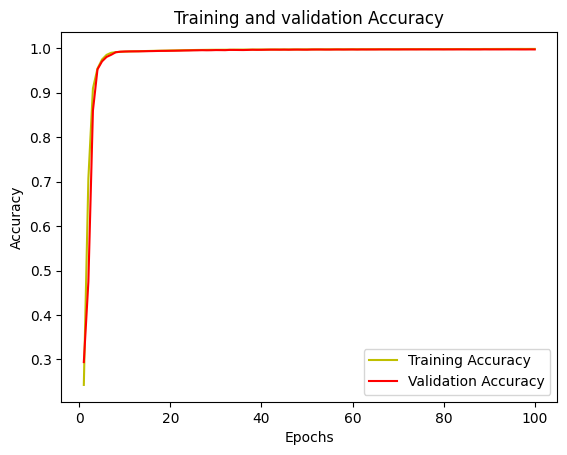
\includegraphics[scale=0.5]{bab4/Rekap Training/VGG16-UNet/mean/4/acc_99,74551796913147.png} &
			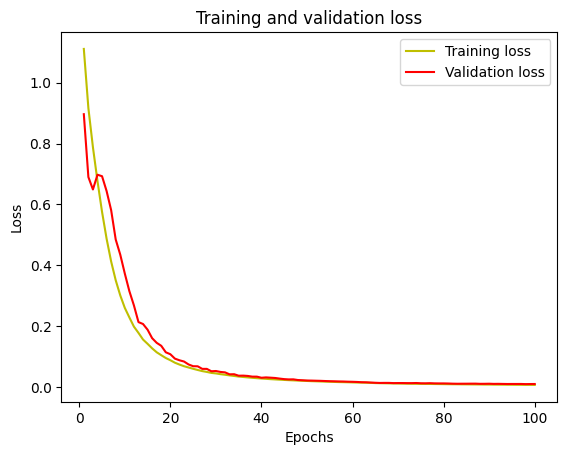
\includegraphics[scale=0.5]{bab4/Rekap Training/VGG16-UNet/mean/4/loss_0,0098.png} & \\
			(a) & (b)    % Caption untuk baris pertama
			% Caption untuk baris kedua
		\end{tabular}
		\caption{Nilai (a) akurasi dan (b) \textit{loss} segmentasi 2D citra \textit{ultrasound} \textit{thrombus} dari hasil citra 3D rekonstruksi yang yang diberi filter \textit{denoising} \textit{mean} menggunakan model \textit{pre-trained} VGG16 dan U-Net.}
		\label{fig:performance-mean-vggunet-rekonstruksi}
	\end{figure}
	
	
	\item \textbf{Filter \textit{denoising} \textit{bilateral}}
	
	Hasil \textit{training} model U-Net yang telah dimodifikasi bagian \textit{encoder}nya menggunakan model \textit{pre-trained} VGG16 dengan menggunakan citra 2D \textit{ultrasound} \textit{thrombus} dari 5 pasien penderita DVT yang melalui tahap reduksi \textit{noise} menggunakan filter \textit{bilateral} diperoleh sebagai berikut, (1) persentase nilai \textit{accuracy} sebesar 99,206\%; (2) nilai \textit{loss} sebesar 0,0267; (3) persentase nilai \textit{mean} IoU sebesar 86,750\%; (4) nilai \textit{mean} \textit{dice coefficient} sebesar 0,8749; serta (5) nilai \textit{mean} \textit{hausdorff distance} sebesar 3,33. Adapun grafik nilai \textit{accuracy} dan nilai \textit{loss} pada proses \textit{training} citra 2D \textit{ultrasound} \textit{thrombus} dari 5 pasien penderita DVT yang melalui tahap reduksi \textit{noise} menggunakan filter \textit{bilateral} dapat dilihat pada Gambar \ref{fig:performance-bilateral-vggunet} bagian a dan b.
	
	
	\begin{figure}[htbp]
		\centering
		\begin{tabular}{ccc}
			% Baris pertama dengan tiga gambar
			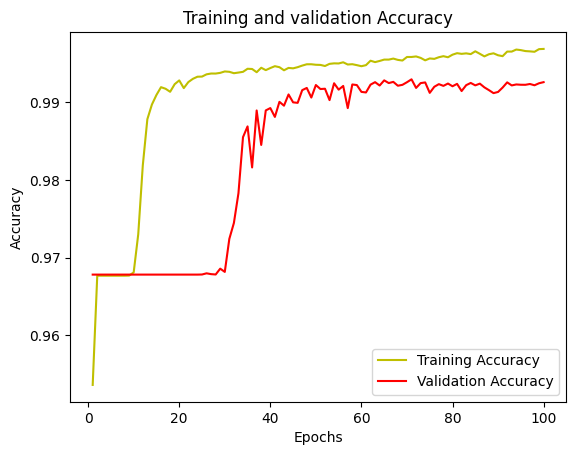
\includegraphics[scale=0.5]{bab4/acc-bilateral-vggunet.png} &
			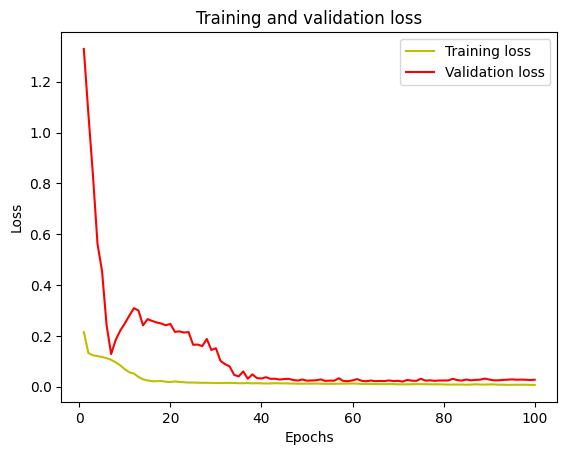
\includegraphics[scale=0.5]{bab4/loss-bilateral-vggunet.png} & \\
			(a) & (b)    % Caption untuk baris pertama
			% Caption untuk baris kedua
		\end{tabular}
		\caption{Nilai (a) akurasi dan (b) \textit{loss} segmentasi model \textit{pre-trained} VGG16-UNet yang menggunakan filter \textit{bilateral}}
		\label{fig:performance-bilateral-vggunet}
	\end{figure}
	
	
	Hasil \textit{training} data 2D citra \textit{ultrasound} \textit{thrombus} dari hasil \textit{slice} citra 3D rekonstruksi yang diberi filter \textit{denoising} \textit{bilateral} menggunakan model \textit{pre-trained} VGG16 dan U-Net diperoleh sebagai berikut, (1) persentase nilai \textit{accuracy} sebesar 99,7051\%; (2) nilai \textit{loss} sebesar 0,0115; (3) nilai \textit{mean} IoU sebesar 0,7518; (4) nilai mean \textit{dice coefficient} sebesar 0,8311; serta (5) nilai \textit{mean hausdorff distance} sebesar 2,5885. Adapun grafik nilai \textit{accuracy} dan nilai \textit{loss} pada proses \textit{training} citra 2D \textit{ultrasound} \textit{thrombus} dari hasil citra 3D rekonstruksi yang diberi filter \textit{denoising} \textit{bilateral} menggunakan model model \textit{pre-trained} VGG16 dan U-Net dapat dilihat pada Gambar \ref{fig:performance-bilateral-vggunet-rekonstruksi}.
	
	
	\begin{figure}[htbp]
		\centering
		\begin{tabular}{ccc}
			% Baris pertama dengan tiga gambar
			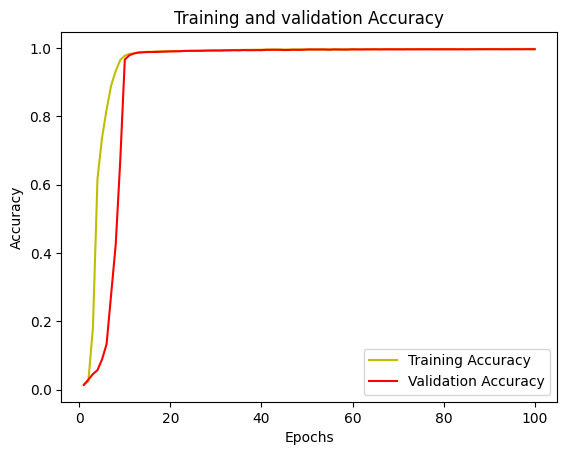
\includegraphics[scale=0.5]{bab4/Rekap Training/VGG16-UNet/bilateral/4/acc_99,64480996131897.png} &
			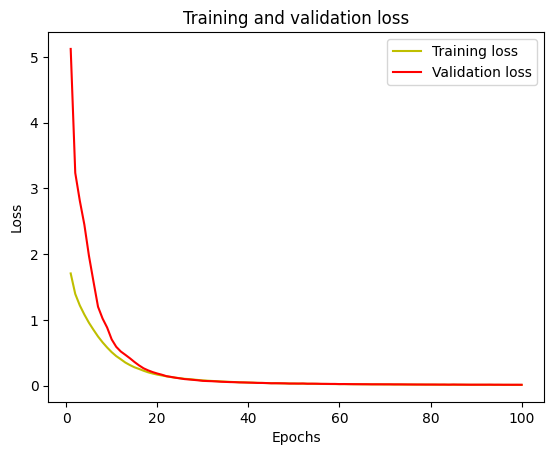
\includegraphics[scale=0.5]{bab4/Rekap Training/VGG16-UNet/bilateral/4/loss_0,0125.png} & \\
			(a) & (b)    % Caption untuk baris pertama
			% Caption untuk baris kedua
		\end{tabular}
		\caption{Nilai (a) akurasi dan (b) \textit{loss} segmentasi 2D citra \textit{ultrasound} \textit{thrombus} dari hasil citra 3D rekonstruksi yang yang diberi filter \textit{denoising} \textit{bilateral} menggunakan model \textit{pre-trained} VGG16 dan U-Net.}
		\label{fig:performance-bilateral-vggunet-rekonstruksi}
	\end{figure}

	\item \textbf{Filter \textit{denoising} \textit{non local means}}
	
	
	Hasil \textit{training} model U-Net yang telah dimodifikasi bagian \textit{encoder}nya menggunakan model \textit{pre-trained} VGG16 dengan menggunakan citra 2D \textit{ultrasound} \textit{thrombus} dari 5 pasien penderita DVT yang melalui tahap reduksi \textit{noise} menggunakan filter \textit{non local means} diperoleh sebagai berikut, (1) persentase nilai \textit{accuracy} sebesar 99,098\%; (2) nilai \textit{loss} sebesar 0,0265; (3) persentase nilai \textit{mean} IoU sebesar 85,516\%; (4) nilai \textit{mean} \textit{dice coefficient} sebesar 0,8520; serta (5) nilai \textit{mean} \textit{hausdorff distance} sebesar 3,49. Adapun grafik nilai \textit{accuracy} dan nilai \textit{loss} pada proses \textit{training} citra 2D \textit{ultrasound} \textit{thrombus} dari 5 pasien penderita DVT yang melalui tahap reduksi \textit{noise} menggunakan filter \textit{non local means} dapat dilihat pada Gambar \ref{fig:performance-nlm-vggunet} bagian a dan b.
	
	
	\begin{figure}[htbp]
		\centering
		\begin{tabular}{ccc}
			% Baris pertama dengan tiga gambar
			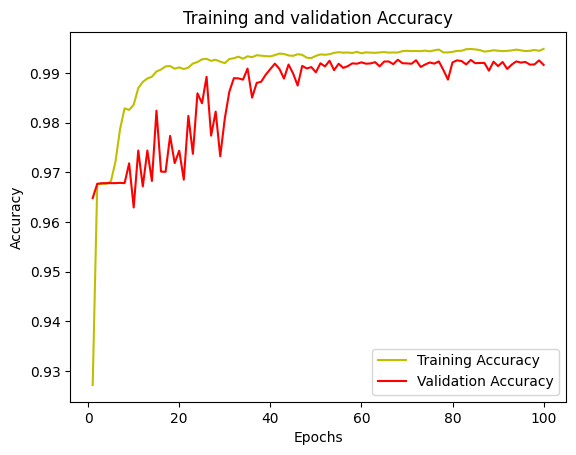
\includegraphics[scale=0.5]{bab4/acc-nlm-vggunet.png} &
			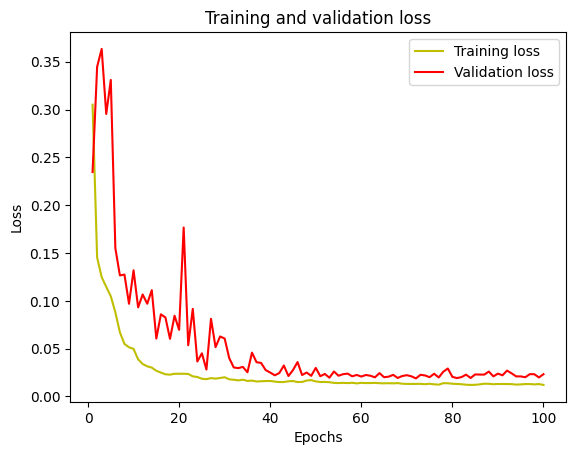
\includegraphics[scale=0.5]{bab4/loss-nlm-vggunet.png} & \\
			(a) & (b)    % Caption untuk baris pertama
			% Caption untuk baris kedua
		\end{tabular}
		\caption{Nilai (a) akurasi dan (b) \textit{loss} segmentasi model \textit{pre-trained} VGG16-UNet yang menggunakan filter \textit{non local means}}
		\label{fig:performance-nlm-vggunet}
	\end{figure}
	
	
	Hasil \textit{training} data 2D citra \textit{ultrasound} \textit{thrombus} dari hasil \textit{slice} citra 3D rekonstruksi yang diberi filter \textit{denoising} \textit{non local means} menggunakan model \textit{pre-trained} VGG16 dan U-Net diperoleh sebagai berikut, (1) persentase nilai \textit{accuracy} sebesar 99,6047\%; (2) nilai \textit{loss} sebesar 0,0118; (3) nilai \textit{mean} IoU sebesar 0,6944; (4) nilai mean \textit{dice coefficient} sebesar 0,7865; serta (5) nilai \textit{mean hausdorff distance} sebesar 6,6529. Adapun grafik nilai \textit{accuracy} dan nilai \textit{loss} pada proses \textit{training} citra 2D \textit{ultrasound} \textit{thrombus} dari hasil citra 3D rekonstruksi yang diberi filter \textit{denoising} \textit{non local means} menggunakan model model \textit{pre-trained} VGG16 dan U-Net dapat dilihat pada Gambar \ref{fig:performance-nlm-vggunet-rekonstruksi}.
	
	
	\begin{figure}[htbp]
		\centering
		\begin{tabular}{ccc}
			% Baris pertama dengan tiga gambar
			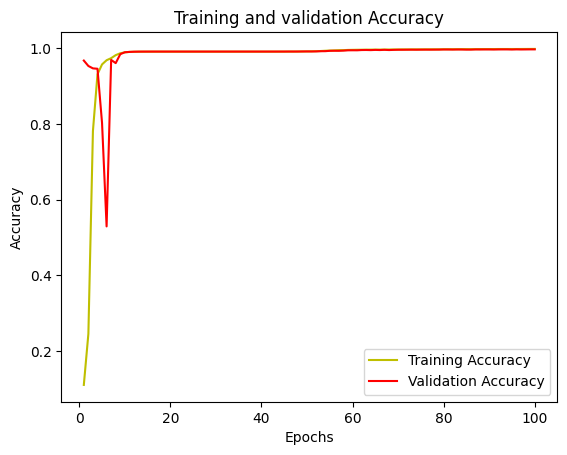
\includegraphics[scale=0.5]{bab4/Rekap Training/VGG16-UNet/nlm/3/acc_99,69685673713684.png} &
			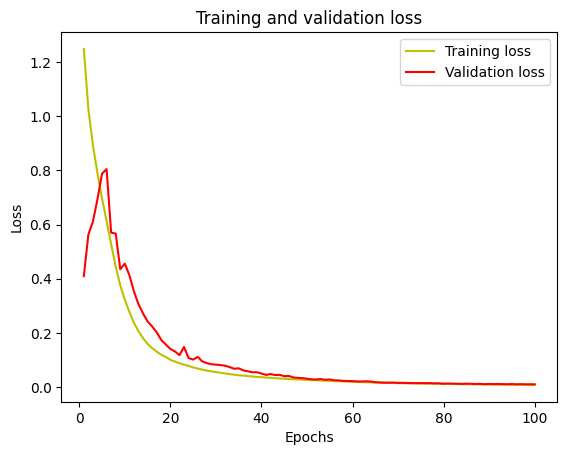
\includegraphics[scale=0.5]{bab4/Rekap Training/VGG16-UNet/nlm/3/loss_0,0106.png} & \\
			(a) & (b)    % Caption untuk baris pertama
			% Caption untuk baris kedua
		\end{tabular}
		\caption{Nilai (a) akurasi dan (b) \textit{loss} segmentasi 2D citra \textit{ultrasound} \textit{thrombus} dari hasil citra 3D rekonstruksi yang yang diberi filter \textit{denoising} \textit{non local means} menggunakan model \textit{pre-trained} VGG16 dan U-Net.}
		\label{fig:performance-nlm-vggunet-rekonstruksi}
	\end{figure}
\end{enumerate}


\subsection{Hasil Performa Segmentasi Citra 2D Thrombus}

Berdasarkan hasil pelatihan (\textit{training}), data citra 2D \textit{ultrasound} \textit{thrombus} pasien DVT dimana sebelumnya telah melalui tahap reduksi \textit{noise} dengan filter \textit{gaussian} serta data citra 2D \textit{ultrasound} \textit{thrombus} dan pembuluh darah hasil \textit{slice} citra 3D hasil rekonstruksi \textit{phantom} balon panjang dimana tanpa melalui tahapan reduksi \textit{noise} yang dilatih menggunakan model segmentasi U-Net standar secara kesuluruhan memberikan performa terbaik dari filter \textit{denoising} yang lain apabila dilihat melalui 5 metrik evaluasi yaitu \textit{accuracy}, \textit{loss}, IoU, \textit{dice coefficient}, dan \textit{hausdorff distance}. Apabila dilihat dari segi \textit{accuracy}, citra 2D \textit{ultrasound} \textit{thrombus} pasien DVT yang direduksi \textit{noise} menggunakan filter \textit{gaussian} serta citra 2D \textit{ultrasound} \textit{thrombus} dan pembuluh darah hasil \textit{slice} citra 3D hasil rekonstruksi \textit{phantom} balon panjang masing - masing mendapat nilai \textit{accuracy} tertinggi yaitu 99,166\% dan 99,7392\%. Kemudian, model U-Net standar yang dikembangkan dari proses \textit{training} citra 2D \textit{ultrasound} \textit{thrombus} pasien DVT tanpa reduksi \textit{noise} serta citra 2D \textit{ultrasound} \textit{thrombus} dan pembuluh darah hasil \textit{slice} citra 3D hasil rekonstruksi \textit{phantom} balon panjang dimana tanpa melalui tahapan reduksi \textit{noise} masing - masing mendapat nilai \textit{loss} terendah sebesar 0,0257 dan 0,0065.

Sementara itu, terdapat 3 metrik evaluasi yang digunakan untuk mengukur tingkat kemiripan antara citra prediksi hasil segmentasi menggunakan model U-Net standar dengan \textit{groundtruth} dari kedua citra 2D tersebut, yaitu IoU, \textit{dice coefficient}, dan \textit{hausdorff distance}. Adapun nilai \textit{mean} IoU tertinggi diperoleh oleh citra 2D \textit{ultrasound} \textit{thrombus} pasien DVT dimana sebelumnya telah melalui tahap reduksi \textit{noise} dengan filter \textit{gaussian} serta citra 2D \textit{ultrasound} \textit{thrombus} dan pembuluh darah hasil \textit{slice} citra 3D hasil rekonstruksi \textit{phantom} balon panjang dimana tanpa melalui tahapan reduksi \textit{noise} masing - masing sebesar 0,7709 dan 0,8174. Kemudian nilai \textit{dice coefficient} tertinggi diperoleh citra 2D \textit{ultrasound} \textit{thrombus} pasien DVT dimana sebelumnya telah melalui tahap reduksi \textit{noise} dengan filter \textit{gaussian} serta citra 2D \textit{ultrasound} \textit{thrombus} dan pembuluh darah hasil \textit{slice} citra 3D hasil rekonstruksi \textit{phantom} balon panjang dimana sebelumnya telah melalui tahap reduksi \textit{noise} dengan filter \textit{mean} masing - masing sebesar 0,8606 dan 0,8925. Sementara itu, nilai \textit{hausdorff distance} terendah diperoleh citra 2D \textit{ultrasound} \textit{thrombus} pasien DVT dimana sebelumnya telah melalui tahap reduksi \textit{noise} dengan filter \textit{gaussian} serta citra 2D \textit{ultrasound} \textit{thrombus} dan pembuluh darah hasil \textit{slice} citra 3D hasil rekonstruksi \textit{phantom} balon panjang dimana tanpa melalui tahapan reduksi \textit{noise} masing - masing sebesar 3,44 dan 3,1244. 

Berdasarkan hasil pelatihan (\textit{training}), citra 2D \textit{ultrasound} \textit{thrombus} pasien DVT dimana sebelumnya telah melalui reduksi noise dengan filter \textit{gaussian} serta citra 2D \textit{ultrasound} \textit{thrombus} dan pembuluh darah hasil \textit{slice} citra 3D hasil rekonstruksi \textit{phantom} balon panjang dimana melalui tahapan reduksi \textit{noise} menggunakan filter median yang masing - masing dilatih menggunakan model segmentasi U-Net yang dimodifikasi \textit{encoder}nya dengan \textit{pre-trained} VGG16 secara keseluruhan memberikan performa terbaik dari filter \textit{denoising} yang lain. Apabila dilihat dari segi \textit{accuracy}, citra 2D \textit{ultrasound} \textit{thrombus} pasien DVT yang melalui tahapan reduksi \textit{noise} dengan filter \textit{gaussian} dan citra 2D \textit{ultrasound} \textit{thrombus} dan pembuluh darah hasil \textit{slice} citra 3D hasil rekonstruksi \textit{phantom} balon panjang yang tidak melalui tahapan reduksi \textit{noise} mendapat nilai \textit{accuracy} tertinggi daripada filter \textit{denoising} yang lain masing - masing sebesar 99,166\% dan 99,7591\%. Kemudian nilai \textit{loss} terendah diperoleh oleh citra 2D \textit{ultrasound} \textit{thrombus} pasien DVT dimana sebelumnya telah melalui reduksi noise dengan filter \textit{mean} dan citra 2D \textit{ultrasound} \textit{thrombus} dan pembuluh darah hasil \textit{slice} citra 3D hasil rekonstruksi \textit{phantom} balon panjang dimana melalui tahapan reduksi \textit{noise} menggunakan filter \textit{gaussian} masing - masing sebesar 0,0256 dan 0,00947.


Kemudian apabila dilihat dari segi 3 metrik evaluasi yang digunakan untuk mengukur tingkat kemiripan antara citra prediksi hasil segmentasi menggunakan model U-Net yang dimodifikasi \textit{encodernya} menggunakan \textit{pre-trained} VGG16 dengan \textit{groundtruth} dari kedua citra 2D tersebut yaitu IoU, \textit{dice coefficient}, dan \textit{hausdorff distance}. Nilai \textit{mean} IoU tertinggi diperoleh oleh citra 2D \textit{ultrasound} \textit{thrombus} pasien DVT dimana sebelumnya telah melalui reduksi noise dengan filter \textit{gaussian} dan citra 2D \textit{ultrasound} \textit{thrombus} dan pembuluh darah hasil \textit{slice} citra 3D hasil rekonstruksi \textit{phantom} balon panjang dimana melalui tahapan reduksi \textit{noise} menggunakan filter \textit{median} dimana masing - masing mendapatkan nilai sebesar 0,8830 dan 0,8336. Kemudian nilai \textit{mean} \textit{dice coefficient} tertinggi diperoleh oleh citra 2D \textit{ultrasound} \textit{thrombus} pasien DVT dimana sebelumnya telah melalui reduksi noise dengan filter \textit{gaussian} dan citra 2D \textit{ultrasound} \textit{thrombus} dan pembuluh darah hasil \textit{slice} citra 3D hasil rekonstruksi \textit{phantom} balon panjang dimana melalui tahapan reduksi \textit{noise} menggunakan filter \textit{median} dengan masing - masing mendapat nilai sebesar 0,8784 dan  0,9049. Sementara itu nilai \textit{hausdorff distance} terendah diperoleh oleh citra 2D \textit{ultrasound} \textit{thrombus} pasien DVT dimana sebelumnya telah melalui reduksi noise dengan filter \textit{gaussian} dan citra 2D \textit{ultrasound} \textit{thrombus} dan pembuluh darah hasil \textit{slice} citra 3D hasil rekonstruksi \textit{phantom} balon panjang dimana melalui tahapan reduksi \textit{noise} menggunakan filter \textit{gaussian} dengan masing - masing sebesar 3,07 dan 1,9526. Hasil performa kedua model segmentasi tersebut dapat dilihat pada Tabel \ref{tab:performa-segmentasi2D}. 


% Please add the following required packages to your document preamble:
% \usepackage{multirow}
% \usepackage{graphicx}
\begin{table}[htbp]
	\centering
	\caption{Performa Segmentasi 2D Citra Ultrasound Pembuluh Darah Dan Thrombus Menggunakan Model Segmentasi U-Net Standar dan U-Net dengan Pre-trained VGG16}
	\label{tab:performa-segmentasi2D}
	\resizebox{\textwidth}{!}{%
		\begin{tabular}{|c|c|c|c|c|c|c|c|}
			\hline
			\textbf{\begin{tabular}[c]{@{}c@{}}Model Segmentasi\\ 2D\end{tabular}}                              & \textbf{Filter Denoising}                 & \textbf{Dataset}                                                                                                                     & \multicolumn{1}{l|}{\textbf{Accuracy}} & \textbf{Loss}    & \textbf{Mean IoU} & \textbf{\begin{tabular}[c]{@{}c@{}}Mean Dice \\ Coefficient\end{tabular}} & \textbf{\begin{tabular}[c]{@{}c@{}}Mean Hausdorff\\ Distance\end{tabular}} \\ \hline
			\multirow{2}{*}{\textbf{U-Net}}                                                                     & \multirow{4}{*}{\textbf{Tanpa Filter}}    & \begin{tabular}[c]{@{}c@{}}Citra 2D ultrasound \\ thrombus pasien DVT\end{tabular}                                                   & 99,021\%                               & \textbf{0,0257}  & 0,7268            & 0,8243                                                                    & 4,12                                                                       \\ \cline{3-8} 
			&                                           & \begin{tabular}[c]{@{}c@{}}Citra 2D ultrasound \\ thrombus dan pembuluh darah \\ hasil slice data citra 3D rekonstruksi\end{tabular} & \textbf{99,7392\%}                     & \textbf{0,0065}  & \textbf{0,8174}   & 0,8923                                                                    & \textbf{3,1244}                                                            \\ \cline{1-1} \cline{3-8} 
			\multirow{2}{*}{\textbf{\begin{tabular}[c]{@{}c@{}}U-Net dengan \\ Pre-trained VGG16\end{tabular}}} &                                           & \begin{tabular}[c]{@{}c@{}}Citra 2D ultrasound \\ thrombus pasien DVT\end{tabular}                                                   & 99,188\%                               & 0,0358           & 0,8709            & 0,8677                                                                    & 3,11                                                                       \\ \cline{3-8} 
			&                                           & \begin{tabular}[c]{@{}c@{}}Citra 2D ultrasound\\ thrombus dan pembuluh darah\\ hasil slice data citra 3D rekonstruksi\end{tabular}   & \textbf{99,7591\%}                     & 0,0103           & 0,8302            & 0,9028                                                                    & 2,0790                                                                     \\ \hline
			\multirow{2}{*}{\textbf{U-Net}}                                                                     & \multirow{4}{*}{\textbf{Gaussian}}        & \begin{tabular}[c]{@{}c@{}}Citra 2D ultrasound \\ thrombus pasien DVT\end{tabular}                                                   & \textbf{99,166\%}                      & 0,0269           & \textbf{0,7709}   & \textbf{0,8606}                                                           & \textbf{3,44}                                                              \\ \cline{3-8} 
			&                                           & \begin{tabular}[c]{@{}c@{}}Citra 2D ultrasound \\ thrombus dan pembuluh darah \\ hasil slice data citra 3D rekonstruksi\end{tabular} & 99,6930\%                              & 0,0074           & 0,7965            & 0,8797                                                                    & 5,0884                                                                     \\ \cline{1-1} \cline{3-8} 
			\multirow{2}{*}{\textbf{\begin{tabular}[c]{@{}c@{}}U-Net dengan \\ Pre-trained VGG16\end{tabular}}} &                                           & \begin{tabular}[c]{@{}c@{}}Citra 2D ultrasound \\ thrombus pasien DVT\end{tabular}                                                   & \textbf{99,222\%}                      & 0,0284           & \textbf{0,8830}   & \textbf{0,8784}                                                           & \textbf{3,07}                                                              \\ \cline{3-8} 
			&                                           & \begin{tabular}[c]{@{}c@{}}Citra 2D ultrasound \\ thrombus dan pembuluh darah \\ hasil slice data citra 3D rekonstruksi\end{tabular} & 99,7489\%                              & \textbf{0,00947} & 0,8267            & 0,9004                                                                    & \textbf{1,9526}                                                            \\ \hline
			\multirow{2}{*}{\textbf{U-Net}}                                                                     & \multirow{4}{*}{\textbf{Median}}          & \begin{tabular}[c]{@{}c@{}}Citra 2D ultrasound \\ thrombus pasien DVT\end{tabular}                                                   & 99,131\%                               & 0,0328           & 0,7572            & 0,8456                                                                    & 3,65                                                                       \\ \cline{3-8} 
			&                                           & \begin{tabular}[c]{@{}c@{}}Citra 2D ultrasound \\ thrombus dan pembuluh darah \\ hasil slice data citra 3D rekonstruksi\end{tabular} & 99,7301\%                              & 0,0067           & 0,8023            & 0,8839                                                                    & 5,0625                                                                     \\ \cline{1-1} \cline{3-8} 
			\multirow{2}{*}{\textbf{\begin{tabular}[c]{@{}c@{}}U-Net dengan \\ Pre-trained VGG16\end{tabular}}} &                                           & \begin{tabular}[c]{@{}c@{}}Citra 2D ultrasound \\ thrombus pasien DVT\end{tabular}                                                   & 99,204\%                               & 0,0353           & 0,8662            & 0,8720                                                                    & 3,12                                                                       \\ \cline{3-8} 
			&                                           & \begin{tabular}[c]{@{}c@{}}Citra 2D ultrasound \\ thrombus dan pembuluh darah \\ hasil slice data citra 3D rekonstruksi\end{tabular} & 99,7512\%                              & 0,00953          & \textbf{0,8336}   & \textbf{0,9049}                                                           & 2,0071                                                                     \\ \hline
			\multirow{2}{*}{\textbf{U-Net}}                                                                     & \multirow{4}{*}{\textbf{Mean}}            & \begin{tabular}[c]{@{}c@{}}Citra 2D ultrasound \\ thrombus pasien DVT\end{tabular}                                                   & 98,374\%                               & 0,0305           & 0,7148            & 0,8570                                                                    & 3,72                                                                       \\ \cline{3-8} 
			&                                           & \begin{tabular}[c]{@{}c@{}}Citra 2D ultrasound \\ thrombus dan pembuluh darah \\ hasil slice data citra 3D rekonstruksi\end{tabular} & 99,7170\%                              & 0,0068           & 0,8147`           & \textbf{0,8925}                                                           & 5,2611                                                                     \\ \cline{1-1} \cline{3-8} 
			\multirow{2}{*}{\textbf{\begin{tabular}[c]{@{}c@{}}U-Net dengan \\ Pre-trained VGG16\end{tabular}}} &                                           & \begin{tabular}[c]{@{}c@{}}Citra 2D ultrasound \\ thrombus pasien DVT\end{tabular}                                                   & 99,218\%                               & \textbf{0,0256}  & 0,8809            & 0,8764                                                                    & 3,48                                                                       \\ \cline{3-8} 
			&                                           & \begin{tabular}[c]{@{}c@{}}Citra 2D ultrasound \\ thrombus dan pembuluh darah \\ hasil slice data citra 3D rekonstruksi\end{tabular} & 99,7480\%                              & 0,0095           & 0,8248            & 0,8992                                                                    & 2,1718                                                                     \\ \hline
			\multirow{2}{*}{\textbf{U-Net}}                                                                     & \multirow{4}{*}{\textbf{Bilateral}}       & \begin{tabular}[c]{@{}c@{}}Citra 2D ultrasound \\ thrombus pasien DVT\end{tabular}                                                   & 98,378\%                               & 0,0267           & 0,7233            & 0,8589                                                                    & 3,58                                                                       \\ \cline{3-8} 
			&                                           & \begin{tabular}[c]{@{}c@{}}Citra 2D ultrasound \\ thrombus dan pembuluh darah \\ hasil slice data citra 3D rekonstruksi\end{tabular} & 99,7318\%                              & 0,0066           & 0,8070            & 0,8872                                                                    & 6,6663                                                                     \\ \cline{1-1} \cline{3-8} 
			\multirow{2}{*}{\textbf{\begin{tabular}[c]{@{}c@{}}U-Net dengan \\ Pre-trained VGG16\end{tabular}}} &                                           & \begin{tabular}[c]{@{}c@{}}Citra 2D ultrasound \\ thrombus pasien DVT\end{tabular}                                                   & 99,206\%                               & 0,0267           & 0,8675            & 0,8749                                                                    & 3,33                                                                       \\ \cline{3-8} 
			&                                           & \begin{tabular}[c]{@{}c@{}}Citra 2D ultrasound \\ thrombus dan pembuluh darah \\ hasil slice data citra 3D rekonstruksi\end{tabular} & 99,7051\%                              & 0,0115           & 0,7518            & 0,8311                                                                    & 2,5885                                                                     \\ \hline
			\multirow{2}{*}{\textbf{U-Net}}                                                                     & \multirow{4}{*}{\textbf{Non Local Means}} & \begin{tabular}[c]{@{}c@{}}Citra 2D ultrasound \\ thrombus pasien DVT\end{tabular}                                                   & 98,381\%                               & 0,0272           & 0,7134            & 0,8599                                                                    & 3,73                                                                       \\ \cline{3-8} 
			&                                           & \begin{tabular}[c]{@{}c@{}}Citra 2D ultrasound \\ thrombus dan pembuluh darah \\ hasil slice data citra 3D rekonstruksi\end{tabular} & 99,6598\%                              & 0,0082           & 0,7819            & 0,8697                                                                    & 4,0778                                                                     \\ \cline{1-1} \cline{3-8} 
			\multirow{2}{*}{\textbf{\begin{tabular}[c]{@{}c@{}}U-Net dengan \\ Pre-trained VGG16\end{tabular}}} &                                           & \begin{tabular}[c]{@{}c@{}}Citra 2D ultrasound \\ thrombus pasien DVT\end{tabular}                                                   & 99,098\%                               & 0,0265           & 0,8552            & 0,8520                                                                    & 3,49                                                                       \\ \cline{3-8} 
			&                                           & \begin{tabular}[c]{@{}c@{}}Citra 2D ultrasound \\ thrombus dan pembuluh darah \\ hasil slice data citra 3D rekonstruksi\end{tabular} & 99,6047\%                              & 0,0118           & 0,6499            & 0,7865                                                                    & 6,6529                                                                     \\ \hline
		\end{tabular}%
	}
\end{table}

Berdasarkan Tabel \ref{tab:performa-segmentasi2D}, secara keseluruhan apabila dilihat dari metrik evaluasi yang digunakan untuk mengukur tingkat kemiripan antara citra prediksi hasil segmentasi dan \textit{groundtruth}, Citra 2D dari hasil segmentasi menggunakan model U-Net dengan \textit{pre-trained} VGG16 memperoleh hasil terbaik daripada citra 2D dari hasil segmentasi menggunakan model U-Net standar. Kemudian filter \textit{gaussian} dan \textit{median} menjadi filter reduksi \textit{noise} terbaik pada segmentasi citra 2D \textit{ultrasound} \textit{thrombus} pasien DVT dan citra 2D \textit{ultrasound} \textit{thrombus} dan pembuluh darah hasil \textit{slice} citra 3D hasil rekonstruksi \textit{phantom} balon panjang. 


Pada pengujian segmentasi area \textit{thrombus} pada citra 2D \textit{ultrasound} penderita DVT menggunakan 5 data citra 2D USG yang telah diberi filter \textit{denoising} \textit{gaussian}. Kelima data tersebut tidak berasal dari data \textit{train} dan data \textit{validation} yang digunakan dalam proses \textit{training}. Hasil perbandingan segmentasi area \textit{thrombus} dari 2 model U-Net yang telah direduksi \textit{noise} dengan filter \textit{gaussian} dapat dilihat pada Gambar \ref{fig:result-label-tabel}.

\begin{figure}[htbp]
	\centering
	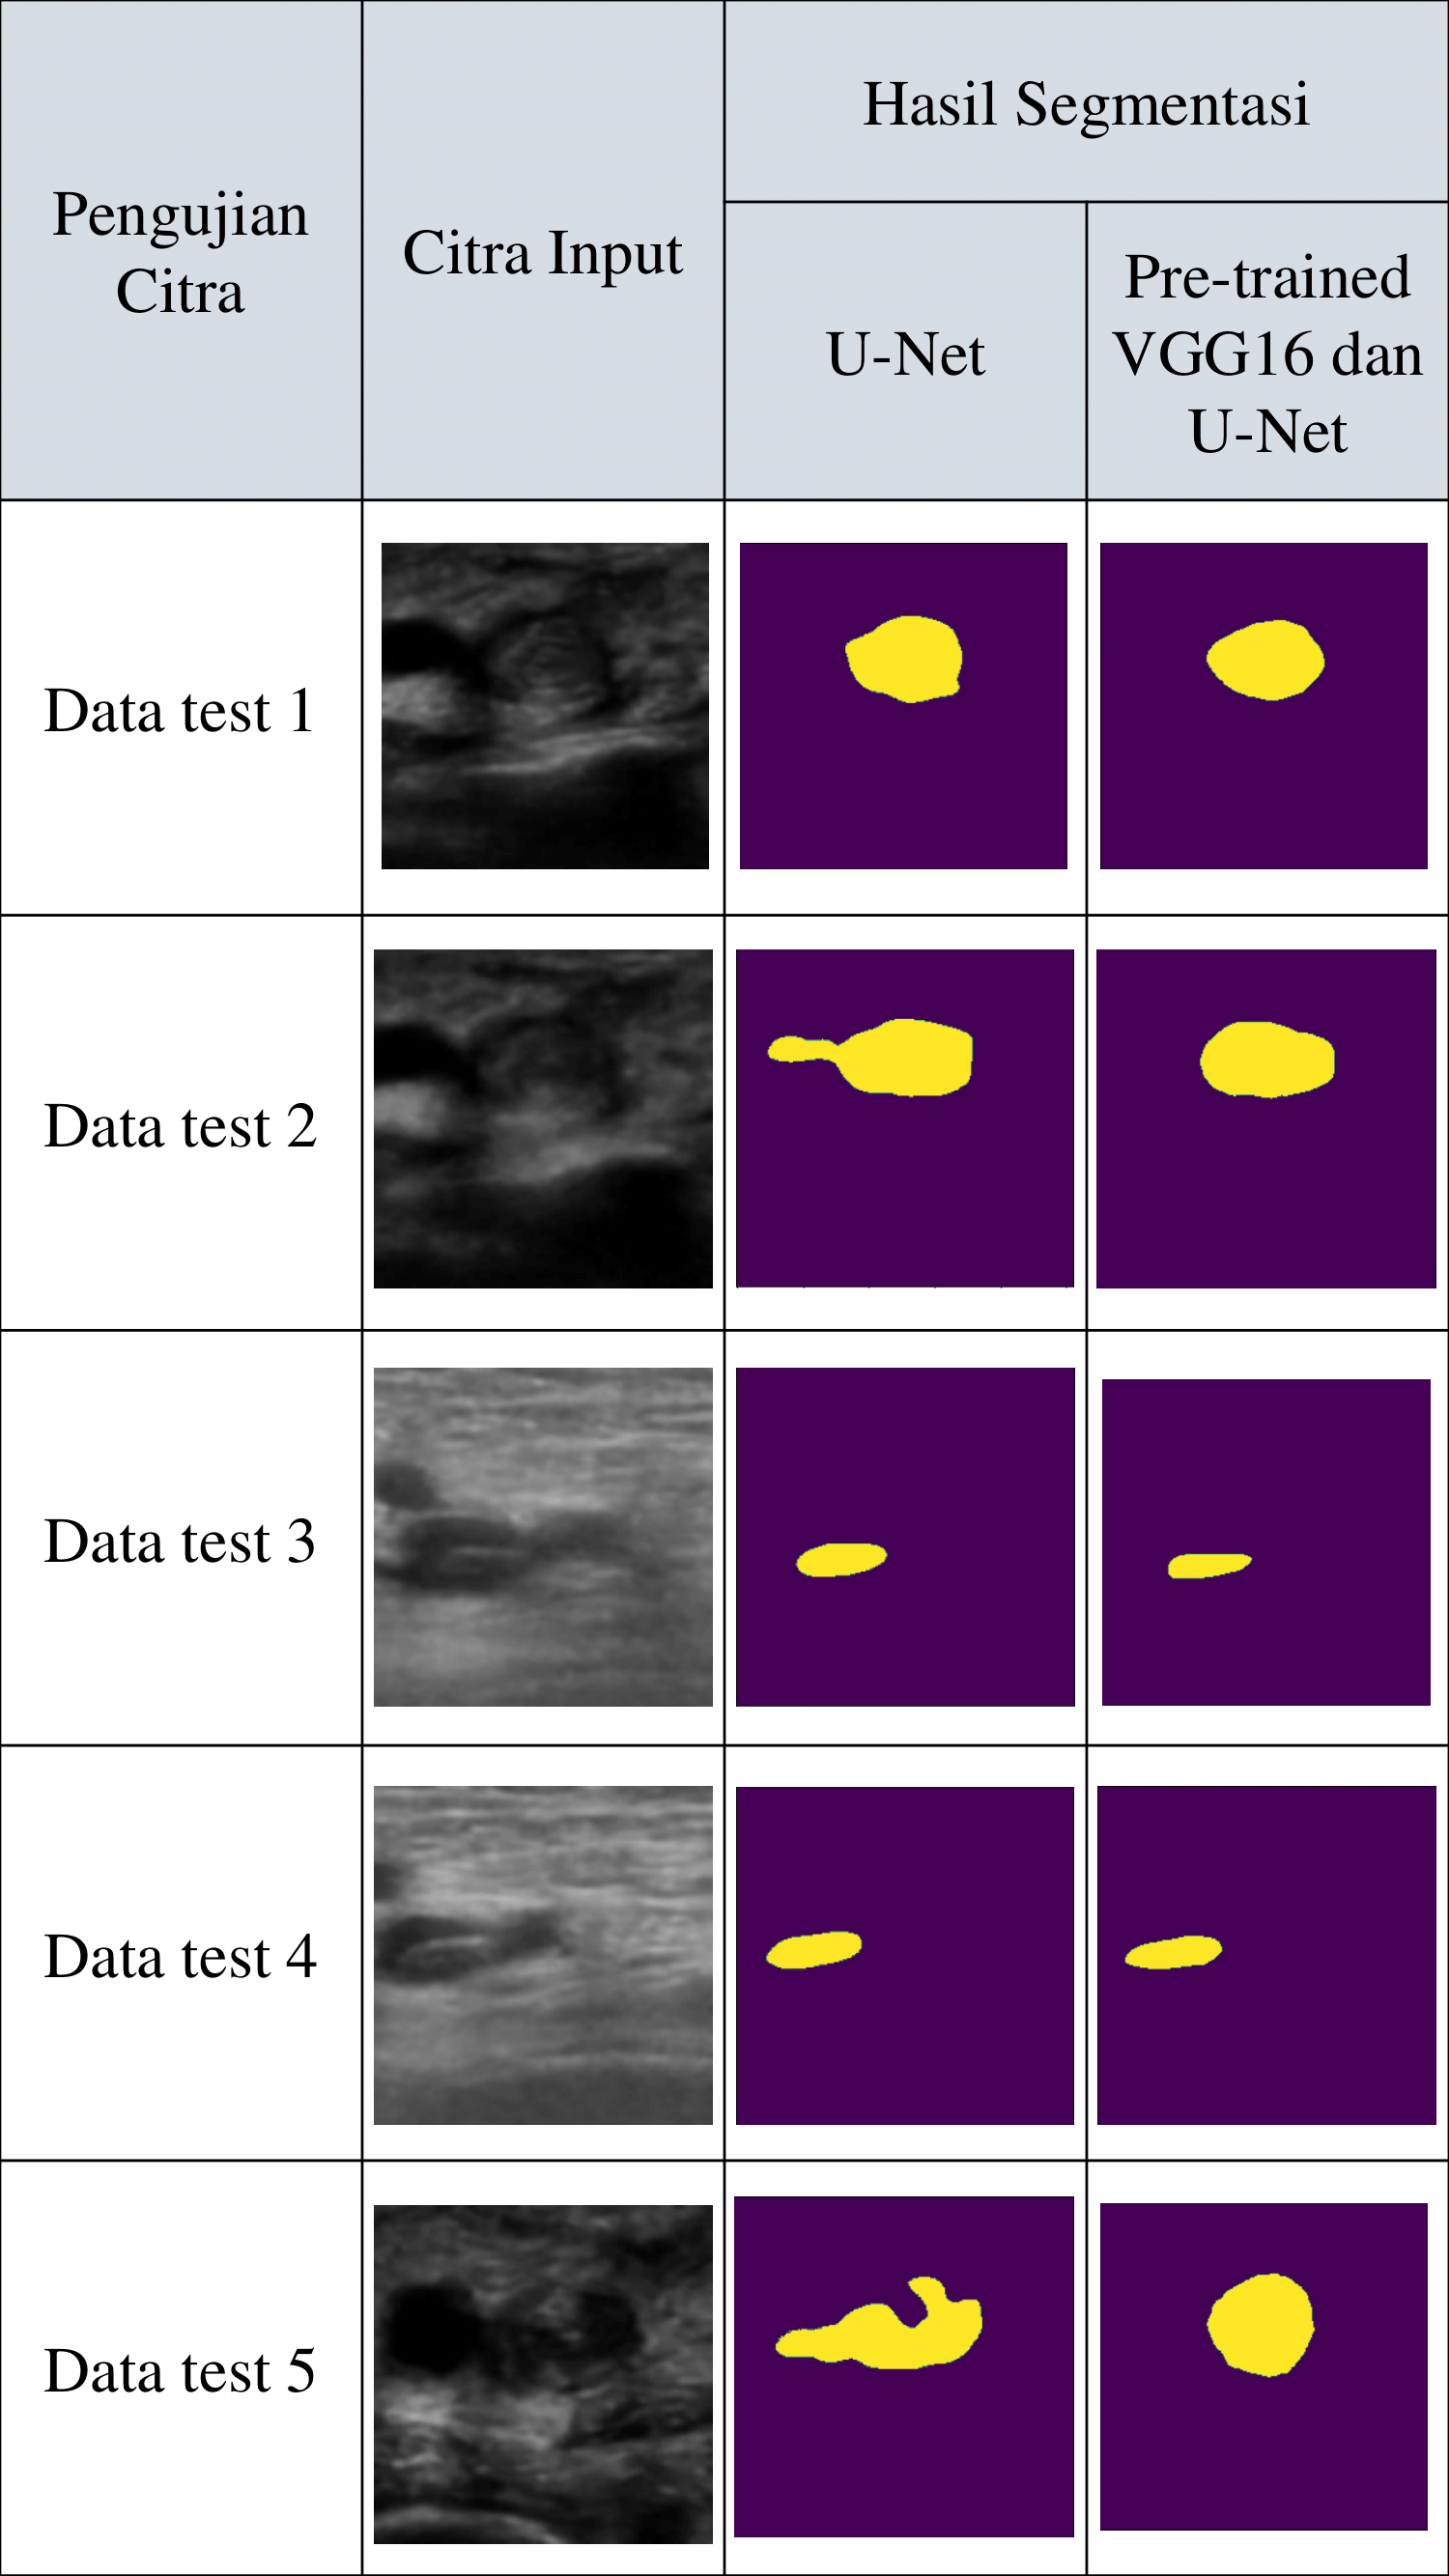
\includegraphics[scale= 0.4]{bab4/Predict_dvt/Predict_dvt-1.png}
	\caption{Perbandingan Hasil Segmentasi Citra 2D \textit{Ultrasound} Penderita DVT}
	\label{fig:result-label-tabel}
\end{figure}

Kemudian, pengujian segmentasi area gumpalan darah \textit{thrombus} pada data 2D citra \textit{ultrasound} dari hasil \textit{slice} citra 3D rekonstruksi \textit{phantom} balon panjang menggunakan 5 data citra 2D \textit{ultrasound} dari hasil \textit{slice} citra 3D rekonstruksi \textit{phantom} balon panjang yang telah diberi filter \textit{denoising} \textit{median}. Kelima data tersebut tidak berasal dari data \textit{train} dan data \textit{validation} yang digunakan dalam proses \textit{training}. Hasil perbandingan segmentasi area \textit{thrombus} pada citra 2D \textit{ultrasound} dari hasil \textit{slice} citra 3D rekonstruksi yang diberi filter \textit{denoising median}  menggunakan model U-Net standar dan model \textit{pre-trained} VGG16 dan U-Net  dapat dilihat pada Gambar \ref{fig:result-label-rekonstruksi}. Adapun area prediksi \textit{thrombus} berwarna kuning, sedangkan area prediksi pembuluh darah berwarna biru.


\begin{figure}[htbp]
	\centering
	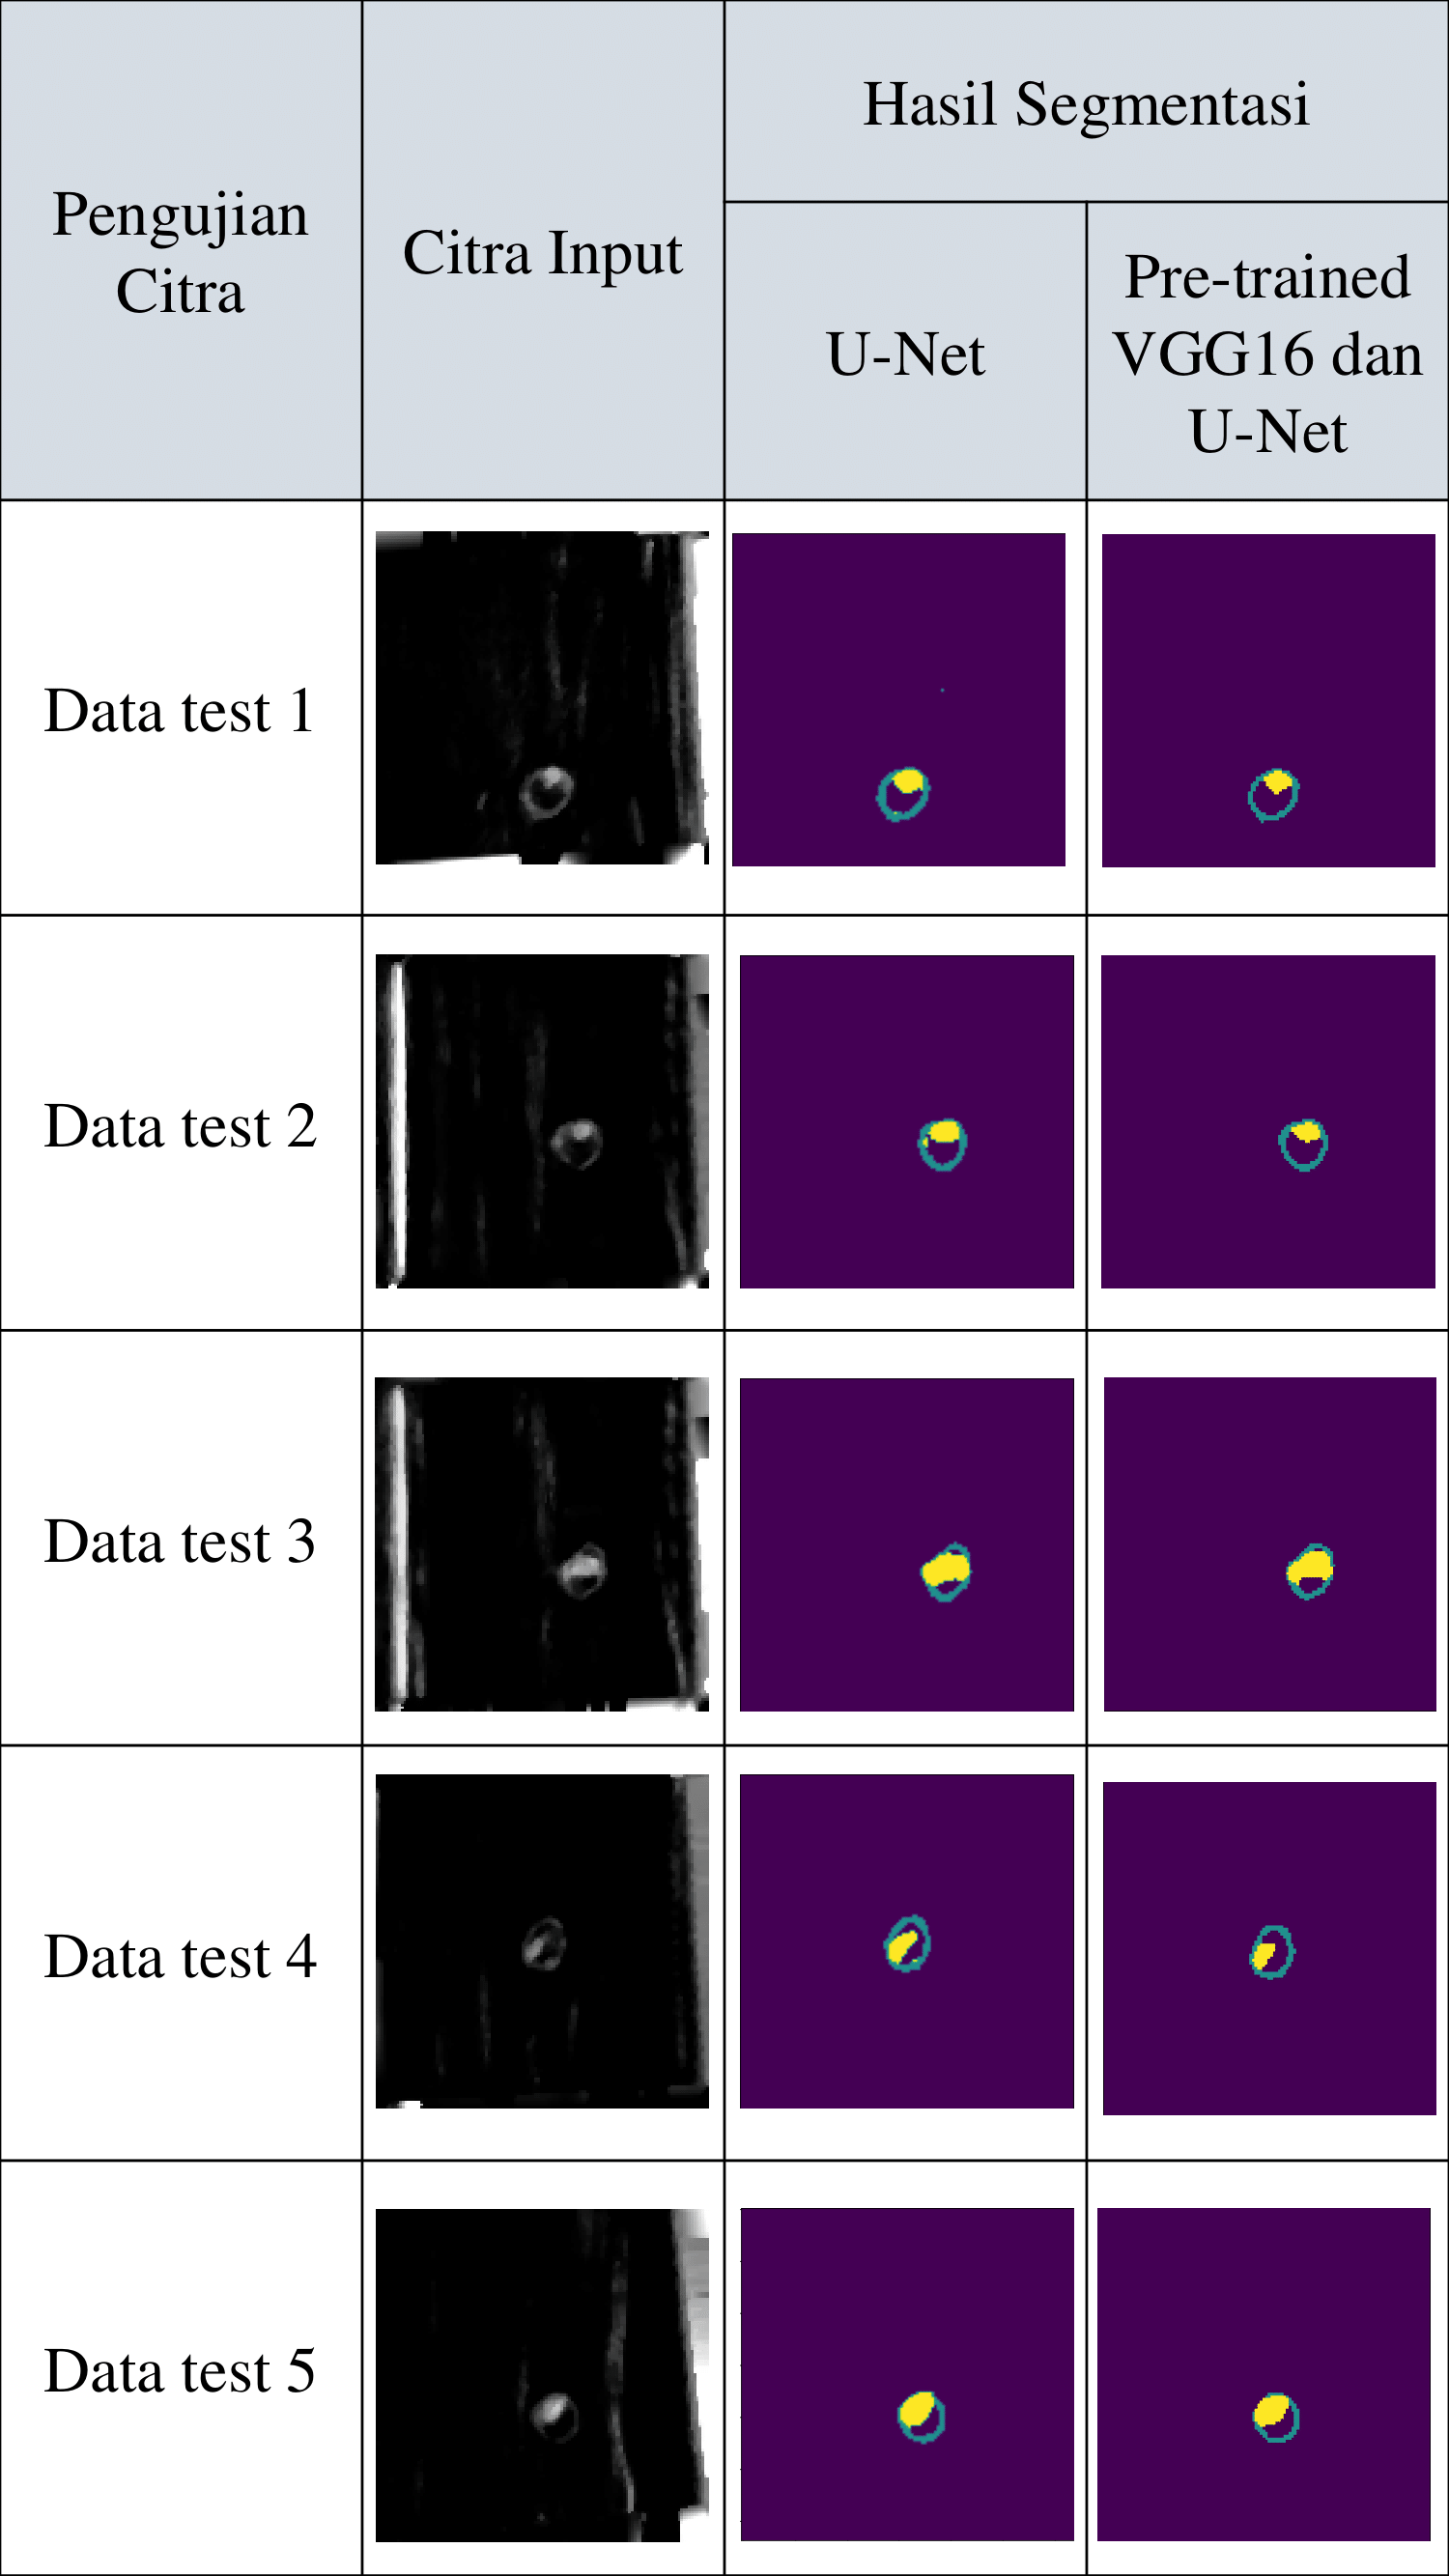
\includegraphics[scale= 0.4]{bab4/result-segmentation_rekonstruksi/result-segmentation_rekonstruksi-1.png}
	\caption{Perbandingan Hasil Segmentasi}
	\label{fig:result-label-rekonstruksi}
\end{figure}



\section{Segmentasi Tiga Dimensi}

\subsection{Persiapan Pengujian}
Pengujian segmentasi 3D pada penelitian ini menggunakan data 3D citra \textit{ultrasound} pembuluh darah dan gumpalan darah (\textit{thrombus}) yang telah direkonstruksi dengan jumlah 4 citra. Sebelum melakukan tahap pelatihan (\textit{training}), citra 3D disamakan ukurannya menjadi 128x128X128. Adapun konfigurasi pengujian pada proses \textit{training} menggunakan model segmentasi 3D menggunakan bahasa pemrograman Python versi 3 yang dijalankan melalui \textit{platform} \textit{Google Colab}, \textit{batch size} didefinisikan sebesar 2, \textit{epoch} 100, inilaisasi \textit{optimizer} menggunakan \textit{Adam} dengan \textit{learning rate} sebesar 0,001, inialisasi \textit{loss} menggunakan \textit{binary crossentropy} dan aktivasi layer pada model menggunakan \textit{softmax}. Adapun hasil segmentasi akan dievaluasi berdasarkan 5 metrik evaluasi yaitu, \textit{accuracy}, \textit{loss}, IoU, \textit{dice coefficient}, dan \textit{hausdorff distance}.

%Pengujian segmentasi 3D pada penelitian ini menggunakan data 3D citra \textit{ultrasound} pembuluh darah dan gumpalan darah (\textit{thrombus}) yang telah direkonstruksi dengan jumlah 5 citra. Data citra tersebut akan melalui tahap reduksi \textit{noise}. Adapun penjelasan terkait reduksi \textit{noise} telah dijelaskan peneliti pada Bab 3.
%
%Kemudian, citra 3D \textit{ultrasound} \textit{thrombus} hasil rekonstruksi yang telah melalui proses reduksi \textit{noise} akan dilakukan proses pelatihan (\textit{training}) data menggunakan model segmentasi 3D U-Net. Penggunaan model 3D U-Net pada proses pelatihan (\textit{training}) berfungsi untuk mengajarkan model tersebut bagaimana mengidentifikasi dan membedakan objek target. Dalam penelitian ini, yang menjadi objek target segmentasi ialah gumpalan darah (\textit{thrombus}) pada pembuluh darah vena. 
%
%Adapun dalam proses segmentasi, penelitian ini menggunakan bahasa pemrograman Python 3 yang dijalankan melalui \textit{platform Google Colab} dengan spesifikasi sebagai berikut (1) \textit{AMD EPYC} 7B12 (2,24 GHz); (2)\textit{RAM} sistem sebesar 12,7 GB; (3)\textit{GPU Tesla T4}; dan memori disk sebesar 166,8 GB. Dalam proses \textit{training} juga ada beberapa konfigurasi yang didefinisikan oleh peneliti sebagai berikut, \textit{batch size} didefinisikan sebesar 2, epoch 100, inialisasi optimizer menggunakan Adam dengan \textit{learning rate} sebesar 0,001, inialisasi \textit{loss} menggunakan \textit{binary crossentropy} dan aktivasi layer pada arsitektur model menggunakan \textit{sigmoid}. Hasil segmentasi akan dievaluasi menggunakan lima \textit{metric} evaluasi sebagai berikut (1)\textit{accuracy}; (2)\textit{loss}; (3)\textit{Intersection over Union} (IoU); (4)\textit{dice coefficient}; dan (5) \textit{hausdorff distance}.
\subsection{\textit{Training} Data 3D Citra \textit{Ultrasound Thrombus} Menggunakan Model Segmentasi U-Net 3D}

%Hasil pengujian \textit{training} model segmentasi menggunakan model U-Net 3D yang digunakan untuk segmentasi citra 3D \textit{ultrasound thrombus}. Data yang digunakan dalam pengujian ini menggunakan data citra 3D \textit{ultrasound thrombus} hasil rekonstruksi. Performa model dinilai berdasarkan 5 metrik evaluasi yaitu \textit{accuracy}, \textit{loss}, IoU, \textit{dice coefficient}, dan \textit{hausdorff distance}. Adapun hasil performa segmentasi 3D citra \textit{ultrasound thrombus} dapat dilihat pada Tabel \ref{tab:performa-segmentasi3D}.

% Please add the following required packages to your document preamble:
% \usepackage{graphicx}



Hasil \textit{training} data 3D citra \textit{ultrasound} pembuluh darah dan \textit{thrombus} menggunakan model segmentasi U-Net 3D diperoleh hasil sebagai berikut, (1) persentase nilai \textit{accuracy} sebesar 99,1078\%; (2) nilai \textit{loss} sebesar 0,0208; (3) nilai mean IoU sebesar 0,8105; (4) nilai \textit{dice coefficient} sebesar 0,8953; dan (5) nilai \textit{hausdorff distance} sebesar .Adapun grafik nilai \textit{accuracy} dan \textit{loss} pada proses \textit{training} citra 3D \textit{ultrasound} pembuluh darah dan \textit{thrombus} menggunakan model U-Net 3D dapat dilihat pada Gambar \ref{fig:performance-unet3d}.

\begin{figure}[htbp]
	\centering
	\begin{tabular}{ccc}
		% Baris pertama dengan tiga gambar
		\includegraphics[scale=0.5]{bab4/segmentasi 3D/acc_99,10783767700195.png} &
		\includegraphics[scale=0.5]{bab4/segmentasi 3D/loss_0,0208.png} & \\
		(a) & (b)    % Caption untuk baris pertama
		% Caption untuk baris kedua
	\end{tabular}
	\caption{Nilai (a) akurasi dan (b) \textit{loss} segmentasi 3D citra \textit{ultrasound} \textit{thrombus} menggunakan model U-Net 3D.}
	\label{fig:performance-unet3d}
\end{figure}



%Pengujian segmentasi 3D pada penelitian ini menggunakan data 3D citra \textit{ultrasound} pembuluh darah dan gumpalan darah (\textit{thrombus}) yang telah direkonstruksi dengan jumlah 5 citra. Data citra tersebut akan melalui tahap reduksi \textit{noise}. Adapun penjelasan terkait reduksi \textit{noise} telah dijelaskan peneliti pada Bab 3.
%
%Kemudian, citra 3D \textit{ultrasound} \textit{thrombus} hasil rekonstruksi yang telah melalui proses reduksi \textit{noise} akan dilakukan proses pelatihan (\textit{training}) data menggunakan model segmentasi 3D U-Net. Penggunaan model 3D U-Net pada proses pelatihan (\textit{training}) berfungsi untuk mengajarkan model tersebut bagaimana mengidentifikasi dan membedakan objek target. Dalam penelitian ini, yang menjadi objek target segmentasi ialah gumpalan darah (\textit{thrombus}) pada pembuluh darah vena. 
%
%Adapun dalam proses segmentasi, penelitian ini menggunakan bahasa pemrograman Python 3 yang dijalankan melalui \textit{platform Google Colab} dengan spesifikasi sebagai berikut (1) \textit{AMD EPYC} 7B12 (2,24 GHz); (2)\textit{RAM} sistem sebesar 12,7 GB; (3)\textit{GPU Tesla T4}; dan memori disk sebesar 166,8 GB. Dalam proses \textit{training} juga ada beberapa konfigurasi yang didefinisikan oleh peneliti sebagai berikut, \textit{batch size} didefinisikan sebesar 2, epoch 100, inialisasi optimizer menggunakan Adam dengan \textit{learning rate} sebesar 0,001, inialisasi \textit{loss} menggunakan \textit{binary crossentropy} dan aktivasi layer pada arsitektur model menggunakan \textit{sigmoid}. Hasil segmentasi akan dievaluasi menggunakan lima \textit{metric} evaluasi sebagai berikut (1)\textit{accuracy}; (2)\textit{loss}; (3)\textit{Intersection over Union} (IoU); (4)\textit{dice coefficient}; dan (5) \textit{hausdorff distance}.
  
\subsection{Hasil Performa Segmentasi Citra 3D Thrombus}

Berdasarkan hasil pelatihan (\textit{training}), Model U-Net 3D memberikan performa terbaik dalam hal \textit{accuracy} dengan nilai . Hal itu menunjukkan bahwa model U-Net 3D tersebut bisa dengan tepat menentukan piksel mana yang menampilkan gumpalan darah \textit{thrombus} dan piksel mana yang tidak. Kemudian model yang dikembangkan dari proses \textit{training}mendapat nilai \textit{loss} sebesar. Hal itu menunjukkan bahwa model segmentasi U-Net 3D dari segi jumlah kesalahan prediksi, model tersebut bekerja paling efektif. Sementara itu terdapat 3 metrik evaluasi yang digunakan untuk mengukur tingkat kemiripan antara citra prediksi hasil segmentasi dengan \textit{groundtruth} dari citra 3D \textit{ultrasound} \textit{thrombus} dan pembuluh darah yang telah direkonstruksi yaitu IoU, \textit{dice coefficient}, dan \textit{hausdorff distance}. Adapun nilai IoU yang diperoleh sebesar 0,8105. Nilai \textit{dice coefficient} sebesar 0,8953. Dan Nilai \textit{hausdorff distance} sebesar 3,25. Hal ini menunjukkan model segmentasi U-Net 3D mampu menghasilkan hasil segmentasi citra prediksi dengan bentuk yang paling dekat dengan bentuk \textit{groundtruth} citra aslinya. Adapun hasil performa segmentasi data 3D \textit{ultrasound} \textit{thrombus} dan pembuluh darah menggunakan model segmentasi U-Net 3D dapat dilihat pada Tabel \ref{tab:performa-segmentasi3D}.

% Please add the following required packages to your document preamble:
% \usepackage{graphicx}
\begin{table}[htbp]
	\centering
	\caption{Performa Segmentasi 3D Citra Ultrasound Pembuluh Darah Dan Thrombus Menggunakan Model Segmentasi U-Net 3D}
	\label{tab:performa-segmentasi3D}
	\resizebox{\textwidth}{!} & 0,0208        & 0,8105            &  0,8953                                                                                         & 3,25                                                                                                \\ \hline
		\end{tabular}%
	}
\end{table}

%Pada pengujian segmentasi 3D area \textit{thrombus} akan menggunakan 4 data citra 3D USG yang berbeda dari data \textit{train} maupun data \textit{validation} yang digunakan dalam proses \textit{training}. Adapun hasil perbandingan segmentasi 3D area \textit{thrombus} dapat dilihat pada Gambar . Diketahui area \textit{thrombus}

Pada pengujian segmentasi 3D area \textit{thrombus} akan menggunakan 4 data citra 3D USG. Adapun hasil perbandingan segmentasi 3D area \textit{thrombus} dapat dilihat pada Gambar \ref{fig:result-label-tabel-segmentasi3d}. Diketahui area \textit{thrombus} berwarna kuning dan area pembuluh darah berwarna biru. Kemudian hasil pengujian performa segmentasi menggunakan model U-Net 3D divisualisasikan dalam bentuk 3D menggunakan perangkat lunak \textit{3D slicer}. Hasil visualisasi 3D hasil segmentasi menggunakan model u-Net 3D dapat dilihat pada Gambar \ref{fig:result-visualize-3D}. Dalam visualisasi 3D tersebut, diketahui \textit{thrombus} ditandai dengan warna merah sedangkan pembuluh darah ditandai dengan warna biru.



\begin{figure}[h]
	\centering
	\includegraphics[scale= 0.2]{bab4/segmentasi 3D/predict_segmentasi3d.png}
	\caption{Perbandingan Hasil Segmentasi}
	\label{fig:result-label-tabel-segmentasi3d}
\end{figure}



\begin{figure}[H]
	\centering
	\begin{tabular}{ccc}
		% Baris pertama dengan tiga gambar
		\includegraphics[width=0.3\textwidth]{bab4/segmentasi 3D/data_test_1.png} &
		\includegraphics[width=0.3\textwidth]{bab4/segmentasi 3D/data_test_2.png}  \\
		(a)  & (b)    \\ % Caption untuk baris pertama
		% Baris kedua dengan tiga gambar
		\includegraphics[width=0.3\textwidth]{bab4/segmentasi 3D/data_test_3.png} &
		\includegraphics[width=0.3\textwidth]{bab4/segmentasi 3D/data_test_4.png} \\
		(c)  & (d)    % Caption untuk baris kedua
	\end{tabular}
	\caption{Visualisasi hasil segmentasi 3D menggunakan model U-Net 3D. (a) Data test 1. (b) Data test 2. (c) Data test 3. (4) Data test 4.}
	\label{fig:result-visualize-3D}
\end{figure}

%\begin{figure}[htbp]
%	\centering
%	\includegraphics[scale= 0.15]{bab4/segmentasi 3D/data_test_2.png}
%	\caption{Perbandingan Hasil Segmentasi}
%	\label{fig:result-label-tabel-segmentasi3d}
%\end{figure}



